\begin{frame}{Reduction from 3-SAT formula}

Clearly this construction is polynomial.  \onslide<+->{\begin{block}{Set k}
 $k = n(q+1) + n-1 + 2q + q-1 + 4
$
\end{block}}

\onslide<+->{\begin{block}{Simplifying}
 $k = 2+2n+(3+n)q$
\end{block}}

\onslide<+->{
\begin{block}{Claim}
$Y$ is satisfiable if and only if $G$ has a path of length of at least $k$.
\end{block}}


\end{frame}

\begin{frame}{Reduction from 3-SAT formula}
\setbeamercovered{dynamic}
\begin{columns}
\begin{column}{0.45\textwidth}
\begin{block}{Necessity}
If $Y$ is satisfiable, then $G$ has a path of length of at least $k$.
\end{block}


  \begin{itemize} 
        \item<1-> Since $Y$ is satisfiable, each clause $c_j$ (where $1 \leq j \leq q$) is true. There must be at least one true literal per clause.
        
\end{itemize}
\end{column}
\begin{column}{0.55\textwidth}
    \begin{overlayarea}{0.55\textwidth}{8cm}
        \only<1->{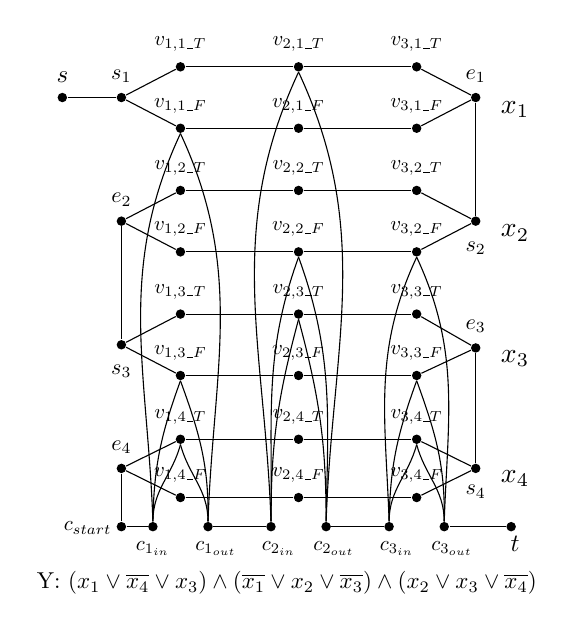
\begin{tikzpicture}[roundnode/.style={circle, fill=black, inner sep=0pt, minimum size=1.2mm}]

    %\foreach \i [count=\ni] in {120,70,...,-180}
        %\node[roundnode] at (\i:1.4cm) (u\ni) {};
    
    \node[roundnode][label=\scalebox{0.9}{${s}$}](u1) at (-1,8.0) {};
    \node[roundnode][label=\scalebox{0.8}{${s_1}$}](u2) at (-0.25,8.0) {};
    \node[roundnode][label=\scalebox{0.75}{${v_{1,1\_T}}$}](u3) at (0.5,8.39) {};
    \node[roundnode][label=\scalebox{0.75}{${v_{1,1\_F}}$}](u4) at (0.5,7.61) {};
    \node[roundnode][label=\scalebox{0.75}{${v_{2,1\_T}}$}](u5) at (2.0,8.39) {};
    \node[roundnode][label=\scalebox{0.75}{${v_{2,1\_F}}$}](u6) at (2.0,7.61) {};
    %\node[roundnode][label=\scalebox{0.75}{${v_{3,1\_T}}$}](u7) at (2.5,8.15) {};
    %\node[roundnode][label=\scalebox{0.75}{${v_{3,1\_F}}$}](u8) at (2.5,7.45) {};
    \node[roundnode][label=\scalebox{0.75}{${v_{3,1\_T}}$}](u9) at (3.5,8.39) {};
    \node[roundnode][label=\scalebox{0.75}{${v_{3,1\_F}}$}](u10) at (3.5,7.61) {};
    \node[roundnode][label=\scalebox{0.8}{$e_1$}](u11) at (4.25,8.0) {};
    \node[style={circle, fill=white, inner sep=0pt, minimum size=0.1mm}][label=\scalebox{1}{$x_1$}](u71) at (4.75, 7.61) {};
    
    \node[roundnode][label=\scalebox{0.8}{${e_2}$}](u12) at (-0.25,6.43) {};
    \node[roundnode][label=\scalebox{0.75}{${v_{1,2\_T}}$}](u13) at (0.5,6.82) {};
    \node[roundnode][label=\scalebox{0.75}{${v_{1,2\_F}}$}](u14) at (0.5,6.04) {};
    \node[roundnode][label=\scalebox{0.75}{${v_{2,2\_T}}$}](u15) at (2.0,6.82) {};
    \node[roundnode][label=\scalebox{0.75}{${v_{2,2\_F}}$}](u16) at (2.0,6.04) {};
    %\node[roundnode][label=\scalebox{0.75}{${v_{3,2\_T}}$}](u17) at (2.5,6.7) {};
    %\node[roundnode][label=\scalebox{0.75}{${v_{3,2\_F}}$}](u18) at (2.5,6) {};
    \node[roundnode][label=\scalebox{0.75}{${v_{3,2\_T}}$}](u19) at (3.5,6.82) {};
    \node[roundnode][label=\scalebox{0.75}{${v_{3,2\_F}}$}](u20) at (3.5,6.04) {};
    \node[roundnode](u21) at (4.25,6.43) {};
    \node[style={circle, fill=white, inner sep=0pt, minimum size=0.2mm}][label=\scalebox{0.8}{$s_2$}](u53) at (4.25, 5.86) {};
    \node[style={circle, fill=white, inner sep=0pt, minimum size=0.1mm}][label=\scalebox{1}{$x_2$}](u72) at (4.75, 6.04) {};
    
    \node[roundnode](u22) at (-0.25,4.86) {};
    \node[style={circle, fill=white, inner sep=0pt, minimum size=0.2mm}][label=\scalebox{0.8}{$s_3$}](u54) at (-0.25, 4.30) {};
    \node[roundnode][label=\scalebox{0.75}{${v_{1,3\_T}}$}](u23) at (0.5,5.25) {};
    \node[roundnode][label=\scalebox{0.75}{${v_{1,3\_F}}$}](u24) at (0.5,4.47) {};
    \node[roundnode][label=\scalebox{0.75}{${v_{2,3\_T}}$}](u25) at (2.0,5.25) {};
    \node[roundnode][label=\scalebox{0.75}{${v_{2,3\_F}}$}](u26) at (2.0,4.47) {};
    %\node[roundnode][label=\scalebox{0.75}{${v_{3,3\_T}}$}](u27) at (2.5,5.25) {};
    %\node[roundnode][label=\scalebox{0.75}{${v_{3,3\_F}}$}](u28) at (2.5,4.55) {};
    \node[roundnode][label=\scalebox{0.75}{${v_{3,3\_T}}$}](u29) at (3.5,5.25) {};
    \node[roundnode][label=\scalebox{0.75}{${v_{3,3\_F}}$}](u30) at (3.5,4.47) {};
    \node[roundnode][label=\scalebox{0.8}{$e_3$}](u31) at (4.25,4.82) {};
    \node[style={circle, fill=white, inner sep=0pt, minimum size=0.1mm}][label=\scalebox{1}{$x_3$}](u73) at (4.75, 4.45) {};
    
    \node[roundnode][label=\scalebox{0.8}{${e_4}$}](u32) at (-0.25,3.29) {};
    \node[roundnode][label=\scalebox{0.75}{${v_{1,4\_T}}$}](u33) at (0.5,3.66) {};
    \node[roundnode][label=\scalebox{0.75}{${v_{1,4\_F}}$}](u34) at (0.5,2.92) {};
    \node[roundnode][label=\scalebox{0.75}{${v_{2,4\_T}}$}](u35) at (2.0,3.66) {};
    \node[roundnode][label=\scalebox{0.75}{${v_{2,4\_F}}$}](u36) at (2.0,2.92) {};
    %\node[roundnode][label=\scalebox{0.75}{${v_{3,4\_T}}$}](u37) at (2.5,3.8) {};
    %\node[roundnode][label=\scalebox{0.75}{${v_{3,4\_F}}$}](u38) at (2.5,3.1) {};
    \node[roundnode][label=\scalebox{0.75}{${v_{3,4\_T}}$}](u39) at (3.5,3.66) {};
    \node[roundnode][label=\scalebox{0.75}{${v_{3,4\_F}}$}](u40) at (3.5,2.92) {};
    \node[roundnode](u41) at (4.25,3.29) {};
    \node[style={circle, fill=white, inner sep=0pt, minimum size=0.2mm}][label=\scalebox{0.8}{$s_4$}](u55) at (4.25, 2.77) {};
    \node[style={circle, fill=white, inner sep=0pt, minimum size=0.1mm}][label=\scalebox{1}{$x_4$}](u74) at (4.75, 2.92) {};
    
    %\node[roundnode](u42) at (-1,3.5) {};
    %\node[roundnode](u43) at (-1,2) {};
    
    \node[roundnode](u43) at (-0.25,2.55) {};
    \node[roundnode](u44) at (0.15,2.55) {};
    \node[roundnode](u45) at (0.85,2.55) {};
    \node[roundnode](u46) at (1.65,2.55) {};
    \node[roundnode](u47) at (2.35,2.55) {};
    %\node[roundnode](u48) at (2.2,2.55) {};
    %\node[roundnode](u49) at (2.8,2.55) {};
    \node[roundnode](u50) at (3.15,2.55) {};
    \node[roundnode](u51) at (3.85,2.55) {};
    
    \node[roundnode](u52) at (4.7,2.55) {};
    \node[style={circle, fill=white, inner sep=0pt, minimum size=0.1mm}][label=\scalebox{0.9}{$t$}](u81) at (4.75, 2.1) {};
    
    \node[style={circle, fill=white, inner sep=0pt, minimum size=0.1mm}][label=\scalebox{0.75}{${c_{1_{in}}}$}](u56) at (0.15,2.05) {};
    \node[style={circle, fill=white, inner sep=0pt, minimum size=0.1mm}][label=\scalebox{0.75}{${c_{1_{out}}}$}](u57) at (0.95,2.05) {};
    \node[style={circle, fill=white, inner sep=0pt, minimum size=0.1mm}][label=\scalebox{0.75}{${c_{2_{in}}}$}](u58) at (1.75,2.05) {};
    \node[style={circle, fill=white, inner sep=0pt, minimum size=0.1mm}][label=\scalebox{0.75}{${c_{2_{out}}}$}](u59) at (2.45,2.05) {};
    \node[style={circle, fill=white, inner sep=0pt, minimum size=0.1mm}][label=\scalebox{0.75}{${c_{3_{in}}}$}](u60) at (3.25,2.05) {};
    \node[style={circle, fill=white, inner sep=0pt, minimum size=0.1mm}][label=\scalebox{0.75}{${c_{3_{out}}}$}](u61) at (3.95,2.05) {};
    
    \node[style={circle, fill=white, inner sep=0pt, minimum size=0.1mm}][label=\scalebox{0.75}{$c_{start}$}](u91) at (-0.68, 2.32) {};
    
            %Lines
            \draw[-] (u1) -- (u2);
            \draw[-] (u2) -- (u3);
            \draw[-] (u2) -- (u4);
            \draw[-] (u3) -- (u5); 
            \draw[-] (u4) -- (u6);
            %\draw[-] (u5) -- (u7);
            %\draw[-] (u6) -- (u8);
            \draw[-] (u5) -- (u9);
            \draw[-] (u6) -- (u10);
            \draw[-] (u9) -- (u11); 
            \draw[-] (u10) -- (u11);
            
            \draw[-] (u11) -- (u21);
            
            \draw[-] (u12) -- (u13);
            \draw[-] (u12) -- (u14);
            \draw[-] (u13) -- (u15); 
            \draw[-] (u14) -- (u16);
            %\draw[-] (u15) -- (u17);
            %\draw[-] (u16) -- (u18);
            \draw[-] (u15) -- (u19);
            \draw[-] (u16) -- (u20);
            \draw[-] (u19) -- (u21); 
            \draw[-] (u20) -- (u21);
            
            \draw[-] (u12) -- (u22);
            
            \draw[-] (u22) -- (u23);
            \draw[-] (u22) -- (u24);
            \draw[-] (u23) -- (u25); 
            \draw[-] (u24) -- (u26);
            %\draw[-] (u25) -- (u27);
            %\draw[-] (u26) -- (u28);
            \draw[-] (u25) -- (u29);
            \draw[-] (u26) -- (u30);
            \draw[-] (u29) -- (u31); 
            \draw[-] (u30) -- (u31);
            
            \draw[-] (u31) -- (u41);
            
            \draw[-] (u32) -- (u33);
            \draw[-] (u32) -- (u34);
            \draw[-] (u33) -- (u35); 
            \draw[-] (u34) -- (u36);
            %\draw[-] (u35) -- (u37);
            %\draw[-] (u36) -- (u38);
            \draw[-] (u35) -- (u39);
            \draw[-] (u36) -- (u40);
            \draw[-] (u39) -- (u41); 
            \draw[-] (u40) -- (u41);
            
            %\draw[-] (u32) -- (u42);
            %\draw[-] (u42) -- (u43);
            \draw[-] (u32) -- (u43);
            \draw[-] (u43) -- (u44); 
            \draw[-] (u45) -- (u46);
            %\draw[-] (u47) -- (u48);
            %\draw[-] (u49) -- (u50);
            \draw[-] (u47) -- (u50);
            \draw[-] (u51) -- (u52);
        
            \begin{scope}
                \draw[-] (u4.south) to [out=245,in=92] (u44.north);
                %(u4) -- (u44);
                \draw[-] (u4.south) to [out=295,in=88] (u45.north);
                \draw[-] (u24.south) to [out=250,in=89] (u44.north);
                \draw[-] (u24.south) to [out=290,in=89] (u45.north);
                \draw[-] (u33.south) to [out=255,in=90] (u44.north);
                \draw[-] (u33.south) to [out=285,in=90] (u45.north);
                
                \draw[-] (u5.south) to [out=245,in=92] (u46.north);
                %(u4) -- (u44);
                \draw[-] (u5.south) to [out=295,in=88] (u47.north);
                \draw[-] (u16.south) to [out=250,in=89] (u46.north);
                \draw[-] (u16.south) to [out=290,in=89] (u47.north);
                \draw[-] (u25.south) to [out=255,in=90] (u46.north);
                \draw[-] (u25.south) to [out=285,in=90] (u47.north);
                
                \draw[-] (u20.south) to [out=245,in=92] (u50.north);
                %(u4) -- (u44);
                \draw[-] (u20.south) to [out=295,in=88] (u51.north);
                \draw[-] (u30.south) to [out=250,in=89] (u50.north);
                \draw[-] (u30.south) to [out=290,in=89] (u51.north);
                \draw[-] (u39.south) to [out=255,in=90] (u50.north);
                \draw[-] (u39.south) to [out=285,in=90] (u51.north);
            \end{scope}
            
    %\node[style={circle, fill=white, inner sep=0pt, minimum size=0.1mm}][label=\scalebox{0.83}{Fig: $Longest Path$ formulation for}](u111) at (2.00, 1.65) {};
    \node[style={circle, fill=white, inner sep=0pt, minimum size=0.1mm}][label=\scalebox{0.83}{Y: $({x_1} \vee \overline{x_4} \vee {x_3}) \wedge (\overline{x_1} \vee{x_2} \vee \overline{x_3}) \wedge
        ({x_2} \vee {x_3} \vee \overline{x_4})$ }](u112) at (1.90, 1.55) {};
        
\end{tikzpicture}
}
    \end{overlayarea}
\end{column}
\end{columns}
\end{frame}

\begin{frame}{Reduction from 3-SAT formula}
\setbeamercovered{dynamic}
\begin{columns}
\begin{column}{0.45\textwidth}
\begin{block}{Necessity}
If $Y$ is satisfiable, then $G$ has a path of length of at least $k$.
\end{block}


  \begin{itemize} 
        \item<1-> Since Y is satisfiable, every variable must have an assignment ($True$ or $False$). So upper path of variable $x_i$ is taken if it is true and lower path is taken if it is false. Thus for every variable, either lower or upper path is taken.
        
\end{itemize}
\end{column}
\begin{column}{0.55\textwidth}
    \begin{overlayarea}{0.55\textwidth}{8cm}
        \only<1->{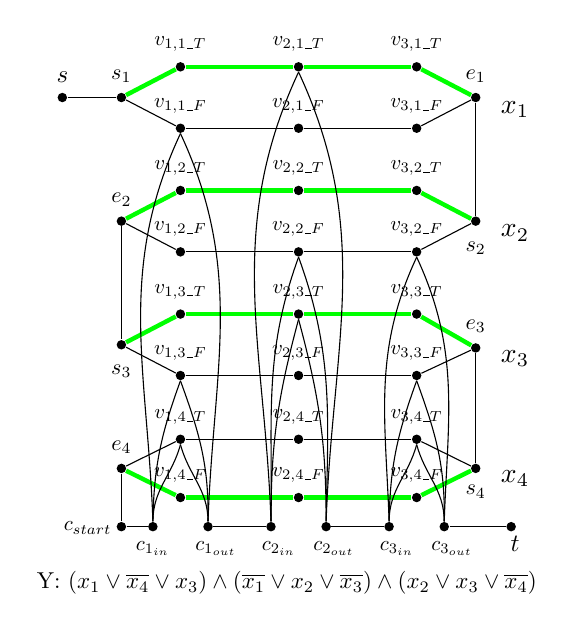
\begin{tikzpicture}[roundnode/.style={circle, fill=black, inner sep=0pt, minimum size=1.2mm}]

    %\foreach \i [count=\ni] in {120,70,...,-180}
        %\node[roundnode] at (\i:1.4cm) (u\ni) {};
    
    \node[roundnode][label=\scalebox{0.9}{${s}$}](u1) at (-1,8.0) {};
    \node[roundnode][label=\scalebox{0.8}{${s_1}$}](u2) at (-0.25,8.0) {};
    \node[roundnode][label=\scalebox{0.75}{${v_{1,1\_T}}$}](u3) at (0.5,8.39) {};
    \node[roundnode][label=\scalebox{0.75}{${v_{1,1\_F}}$}](u4) at (0.5,7.61) {};
    \node[roundnode][label=\scalebox{0.75}{${v_{2,1\_T}}$}](u5) at (2.0,8.39) {};
    \node[roundnode][label=\scalebox{0.75}{${v_{2,1\_F}}$}](u6) at (2.0,7.61) {};
    %\node[roundnode][label=\scalebox{0.75}{${v_{3,1\_T}}$}](u7) at (2.5,8.15) {};
    %\node[roundnode][label=\scalebox{0.75}{${v_{3,1\_F}}$}](u8) at (2.5,7.45) {};
    \node[roundnode][label=\scalebox{0.75}{${v_{3,1\_T}}$}](u9) at (3.5,8.39) {};
    \node[roundnode][label=\scalebox{0.75}{${v_{3,1\_F}}$}](u10) at (3.5,7.61) {};
    \node[roundnode][label=\scalebox{0.8}{$e_1$}](u11) at (4.25,8.0) {};
    \node[style={circle, fill=white, inner sep=0pt, minimum size=0.1mm}][label=\scalebox{1}{$x_1$}](u71) at (4.75, 7.61) {};
    
    \node[roundnode][label=\scalebox{0.8}{${e_2}$}](u12) at (-0.25,6.43) {};
    \node[roundnode][label=\scalebox{0.75}{${v_{1,2\_T}}$}](u13) at (0.5,6.82) {};
    \node[roundnode][label=\scalebox{0.75}{${v_{1,2\_F}}$}](u14) at (0.5,6.04) {};
    \node[roundnode][label=\scalebox{0.75}{${v_{2,2\_T}}$}](u15) at (2.0,6.82) {};
    \node[roundnode][label=\scalebox{0.75}{${v_{2,2\_F}}$}](u16) at (2.0,6.04) {};
    %\node[roundnode][label=\scalebox{0.75}{${v_{3,2\_T}}$}](u17) at (2.5,6.7) {};
    %\node[roundnode][label=\scalebox{0.75}{${v_{3,2\_F}}$}](u18) at (2.5,6) {};
    \node[roundnode][label=\scalebox{0.75}{${v_{3,2\_T}}$}](u19) at (3.5,6.82) {};
    \node[roundnode][label=\scalebox{0.75}{${v_{3,2\_F}}$}](u20) at (3.5,6.04) {};
    \node[roundnode](u21) at (4.25,6.43) {};
    \node[style={circle, fill=white, inner sep=0pt, minimum size=0.2mm}][label=\scalebox{0.8}{$s_2$}](u53) at (4.25, 5.86) {};
    \node[style={circle, fill=white, inner sep=0pt, minimum size=0.1mm}][label=\scalebox{1}{$x_2$}](u72) at (4.75, 6.04) {};
    
    \node[roundnode](u22) at (-0.25,4.86) {};
    \node[style={circle, fill=white, inner sep=0pt, minimum size=0.2mm}][label=\scalebox{0.8}{$s_3$}](u54) at (-0.25, 4.30) {};
    \node[roundnode][label=\scalebox{0.75}{${v_{1,3\_T}}$}](u23) at (0.5,5.25) {};
    \node[roundnode][label=\scalebox{0.75}{${v_{1,3\_F}}$}](u24) at (0.5,4.47) {};
    \node[roundnode][label=\scalebox{0.75}{${v_{2,3\_T}}$}](u25) at (2.0,5.25) {};
    \node[roundnode][label=\scalebox{0.75}{${v_{2,3\_F}}$}](u26) at (2.0,4.47) {};
    %\node[roundnode][label=\scalebox{0.75}{${v_{3,3\_T}}$}](u27) at (2.5,5.25) {};
    %\node[roundnode][label=\scalebox{0.75}{${v_{3,3\_F}}$}](u28) at (2.5,4.55) {};
    \node[roundnode][label=\scalebox{0.75}{${v_{3,3\_T}}$}](u29) at (3.5,5.25) {};
    \node[roundnode][label=\scalebox{0.75}{${v_{3,3\_F}}$}](u30) at (3.5,4.47) {};
    \node[roundnode][label=\scalebox{0.8}{$e_3$}](u31) at (4.25,4.82) {};
    \node[style={circle, fill=white, inner sep=0pt, minimum size=0.1mm}][label=\scalebox{1}{$x_3$}](u73) at (4.75, 4.45) {};
    
    \node[roundnode][label=\scalebox{0.8}{${e_4}$}](u32) at (-0.25,3.29) {};
    \node[roundnode][label=\scalebox{0.75}{${v_{1,4\_T}}$}](u33) at (0.5,3.66) {};
    \node[roundnode][label=\scalebox{0.75}{${v_{1,4\_F}}$}](u34) at (0.5,2.92) {};
    \node[roundnode][label=\scalebox{0.75}{${v_{2,4\_T}}$}](u35) at (2.0,3.66) {};
    \node[roundnode][label=\scalebox{0.75}{${v_{2,4\_F}}$}](u36) at (2.0,2.92) {};
    %\node[roundnode][label=\scalebox{0.75}{${v_{3,4\_T}}$}](u37) at (2.5,3.8) {};
    %\node[roundnode][label=\scalebox{0.75}{${v_{3,4\_F}}$}](u38) at (2.5,3.1) {};
    \node[roundnode][label=\scalebox{0.75}{${v_{3,4\_T}}$}](u39) at (3.5,3.66) {};
    \node[roundnode][label=\scalebox{0.75}{${v_{3,4\_F}}$}](u40) at (3.5,2.92) {};
    \node[roundnode](u41) at (4.25,3.29) {};
    \node[style={circle, fill=white, inner sep=0pt, minimum size=0.2mm}][label=\scalebox{0.8}{$s_4$}](u55) at (4.25, 2.77) {};
    \node[style={circle, fill=white, inner sep=0pt, minimum size=0.1mm}][label=\scalebox{1}{$x_4$}](u74) at (4.75, 2.92) {};
    
    %\node[roundnode](u42) at (-1,3.5) {};
    %\node[roundnode](u43) at (-1,2) {};
    
    \node[roundnode](u43) at (-0.25,2.55) {};
    \node[roundnode](u44) at (0.15,2.55) {};
    \node[roundnode](u45) at (0.85,2.55) {};
    \node[roundnode](u46) at (1.65,2.55) {};
    \node[roundnode](u47) at (2.35,2.55) {};
    %\node[roundnode](u48) at (2.2,2.55) {};
    %\node[roundnode](u49) at (2.8,2.55) {};
    \node[roundnode](u50) at (3.15,2.55) {};
    \node[roundnode](u51) at (3.85,2.55) {};
    
    \node[roundnode](u52) at (4.7,2.55) {};
    \node[style={circle, fill=white, inner sep=0pt, minimum size=0.1mm}][label=\scalebox{0.9}{$t$}](u81) at (4.75, 2.1) {};
    
    \node[style={circle, fill=white, inner sep=0pt, minimum size=0.1mm}][label=\scalebox{0.75}{${c_{1_{in}}}$}](u56) at (0.15,2.05) {};
    \node[style={circle, fill=white, inner sep=0pt, minimum size=0.1mm}][label=\scalebox{0.75}{${c_{1_{out}}}$}](u57) at (0.95,2.05) {};
    \node[style={circle, fill=white, inner sep=0pt, minimum size=0.1mm}][label=\scalebox{0.75}{${c_{2_{in}}}$}](u58) at (1.75,2.05) {};
    \node[style={circle, fill=white, inner sep=0pt, minimum size=0.1mm}][label=\scalebox{0.75}{${c_{2_{out}}}$}](u59) at (2.45,2.05) {};
    \node[style={circle, fill=white, inner sep=0pt, minimum size=0.1mm}][label=\scalebox{0.75}{${c_{3_{in}}}$}](u60) at (3.25,2.05) {};
    \node[style={circle, fill=white, inner sep=0pt, minimum size=0.1mm}][label=\scalebox{0.75}{${c_{3_{out}}}$}](u61) at (3.95,2.05) {};
    
    \node[style={circle, fill=white, inner sep=0pt, minimum size=0.1mm}][label=\scalebox{0.75}{$c_{start}$}](u91) at (-0.68, 2.32) {};
    
            %Lines
            \draw[-] (u1) -- (u2);
            \draw[-, ultra thick, green] (u2) -- (u3);
            \draw[-] (u2) -- (u4);
            \draw[-, ultra thick,green] (u3) -- (u5); 
            \draw[-] (u4) -- (u6);
            %\draw[-] (u5) -- (u7);
            %\draw[-] (u6) -- (u8);
            \draw[-,ultra thick, green] (u5) -- (u9);
            \draw[-] (u6) -- (u10);
            \draw[-, ultra thick, green] (u9) -- (u11); 
            \draw[-] (u10) -- (u11);
            
            \draw[-] (u11) -- (u21);
            
            \draw[-, ultra thick, green] (u12) -- (u13);
            \draw[-] (u12) -- (u14);
            \draw[-, ultra thick, green] (u13) -- (u15); 
            \draw[-] (u14) -- (u16);
            %\draw[-] (u15) -- (u17);
            %\draw[-] (u16) -- (u18);
            \draw[-, ultra thick, green] (u15) -- (u19);
            \draw[-] (u16) -- (u20);
            \draw[-, ultra thick, green] (u19) -- (u21); 
            \draw[-] (u20) -- (u21);
            
            \draw[-] (u12) -- (u22);
            
            \draw[-, ultra thick, green] (u22) -- (u23);
            \draw[-] (u22) -- (u24);
            \draw[-, ultra thick, green] (u23) -- (u25); 
            \draw[-] (u24) -- (u26);
            %\draw[-] (u25) -- (u27);
            %\draw[-] (u26) -- (u28);
            \draw[-, ultra thick, green] (u25) -- (u29);
            \draw[-] (u26) -- (u30);
            \draw[-, ultra thick, green] (u29) -- (u31); 
            \draw[-] (u30) -- (u31);
            
            \draw[-] (u31) -- (u41);
            
            \draw[-] (u32) -- (u33);
            \draw[-, ultra thick, green] (u32) -- (u34);
            \draw[-] (u33) -- (u35); 
            \draw[-, ultra thick, green] (u34) -- (u36);
            %\draw[-] (u35) -- (u37);
            %\draw[-] (u36) -- (u38);
            \draw[-] (u35) -- (u39);
            \draw[-, ultra thick, green] (u36) -- (u40);
            \draw[-] (u39) -- (u41); 
            \draw[-, ultra thick, green] (u40) -- (u41);
            
            %\draw[-] (u32) -- (u42);
            %\draw[-] (u42) -- (u43);
            \draw[-] (u32) -- (u43);
            \draw[-] (u43) -- (u44); 
            \draw[-] (u45) -- (u46);
            %\draw[-] (u47) -- (u48);
            %\draw[-] (u49) -- (u50);
            \draw[-] (u47) -- (u50);
            \draw[-] (u51) -- (u52);
        
            \begin{scope}
                \draw[-] (u4.south) to [out=245,in=92] (u44.north);
                %(u4) -- (u44);
                \draw[-] (u4.south) to [out=295,in=88] (u45.north);
                \draw[-] (u24.south) to [out=250,in=89] (u44.north);
                \draw[-] (u24.south) to [out=290,in=89] (u45.north);
                \draw[-] (u33.south) to [out=255,in=90] (u44.north);
                \draw[-] (u33.south) to [out=285,in=90] (u45.north);
                
                \draw[-] (u5.south) to [out=245,in=92] (u46.north);
                %(u4) -- (u44);
                \draw[-] (u5.south) to [out=295,in=88] (u47.north);
                \draw[-] (u16.south) to [out=250,in=89] (u46.north);
                \draw[-] (u16.south) to [out=290,in=89] (u47.north);
                \draw[-] (u25.south) to [out=255,in=90] (u46.north);
                \draw[-] (u25.south) to [out=285,in=90] (u47.north);
                
                \draw[-] (u20.south) to [out=245,in=92] (u50.north);
                %(u4) -- (u44);
                \draw[-] (u20.south) to [out=295,in=88] (u51.north);
                \draw[-] (u30.south) to [out=250,in=89] (u50.north);
                \draw[-] (u30.south) to [out=290,in=89] (u51.north);
                \draw[-] (u39.south) to [out=255,in=90] (u50.north);
                \draw[-] (u39.south) to [out=285,in=90] (u51.north);
            \end{scope}
        \node[style={circle, fill=white, inner sep=0pt, minimum size=0.1mm}][label=\scalebox{0.83}{Y: $({x_1} \vee \overline{x_4} \vee {x_3}) \wedge (\overline{x_1} \vee{x_2} \vee \overline{x_3}) \wedge
        ({x_2} \vee {x_3} \vee \overline{x_4})$ }](u112) at (1.90, 1.55) {};
            
\end{tikzpicture}}
    \end{overlayarea}
\end{column}
\end{columns}
\end{frame}

\begin{frame}{Reduction from 3-SAT formula}
\setbeamercovered{dynamic}
\begin{columns}
\begin{column}{0.45\textwidth}
\begin{block}{Necessity}
If $Y$ is satisfiable, then $G$ has a path of length of at least $k$.
\end{block}

  \begin{itemize} 
    \item<1->Length of a path between the start and the end vertex in one loop is $q+1$. Thus total $n*(q+1)$ edges are taken.
    \item<2-> To construct a path, we need to take edges from ending vertex of each loop to starting vertex of next loop. 
    \item<3->So total $n-1$ edges are taken.

\end{itemize}
\end{column}
\begin{column}{0.55\textwidth}
    \begin{overlayarea}{0.55\textwidth}{8cm}
        \only<1>{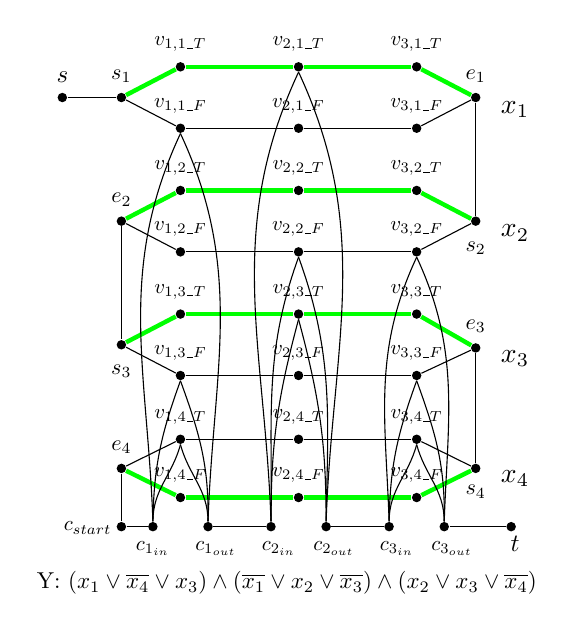
\begin{tikzpicture}[roundnode/.style={circle, fill=black, inner sep=0pt, minimum size=1.2mm}]

    %\foreach \i [count=\ni] in {120,70,...,-180}
        %\node[roundnode] at (\i:1.4cm) (u\ni) {};
    
    \node[roundnode][label=\scalebox{0.9}{${s}$}](u1) at (-1,8.0) {};
    \node[roundnode][label=\scalebox{0.8}{${s_1}$}](u2) at (-0.25,8.0) {};
    \node[roundnode][label=\scalebox{0.75}{${v_{1,1\_T}}$}](u3) at (0.5,8.39) {};
    \node[roundnode][label=\scalebox{0.75}{${v_{1,1\_F}}$}](u4) at (0.5,7.61) {};
    \node[roundnode][label=\scalebox{0.75}{${v_{2,1\_T}}$}](u5) at (2.0,8.39) {};
    \node[roundnode][label=\scalebox{0.75}{${v_{2,1\_F}}$}](u6) at (2.0,7.61) {};
    %\node[roundnode][label=\scalebox{0.75}{${v_{3,1\_T}}$}](u7) at (2.5,8.15) {};
    %\node[roundnode][label=\scalebox{0.75}{${v_{3,1\_F}}$}](u8) at (2.5,7.45) {};
    \node[roundnode][label=\scalebox{0.75}{${v_{3,1\_T}}$}](u9) at (3.5,8.39) {};
    \node[roundnode][label=\scalebox{0.75}{${v_{3,1\_F}}$}](u10) at (3.5,7.61) {};
    \node[roundnode][label=\scalebox{0.8}{$e_1$}](u11) at (4.25,8.0) {};
    \node[style={circle, fill=white, inner sep=0pt, minimum size=0.1mm}][label=\scalebox{1}{$x_1$}](u71) at (4.75, 7.61) {};
    
    \node[roundnode][label=\scalebox{0.8}{${e_2}$}](u12) at (-0.25,6.43) {};
    \node[roundnode][label=\scalebox{0.75}{${v_{1,2\_T}}$}](u13) at (0.5,6.82) {};
    \node[roundnode][label=\scalebox{0.75}{${v_{1,2\_F}}$}](u14) at (0.5,6.04) {};
    \node[roundnode][label=\scalebox{0.75}{${v_{2,2\_T}}$}](u15) at (2.0,6.82) {};
    \node[roundnode][label=\scalebox{0.75}{${v_{2,2\_F}}$}](u16) at (2.0,6.04) {};
    %\node[roundnode][label=\scalebox{0.75}{${v_{3,2\_T}}$}](u17) at (2.5,6.7) {};
    %\node[roundnode][label=\scalebox{0.75}{${v_{3,2\_F}}$}](u18) at (2.5,6) {};
    \node[roundnode][label=\scalebox{0.75}{${v_{3,2\_T}}$}](u19) at (3.5,6.82) {};
    \node[roundnode][label=\scalebox{0.75}{${v_{3,2\_F}}$}](u20) at (3.5,6.04) {};
    \node[roundnode](u21) at (4.25,6.43) {};
    \node[style={circle, fill=white, inner sep=0pt, minimum size=0.2mm}][label=\scalebox{0.8}{$s_2$}](u53) at (4.25, 5.86) {};
    \node[style={circle, fill=white, inner sep=0pt, minimum size=0.1mm}][label=\scalebox{1}{$x_2$}](u72) at (4.75, 6.04) {};
    
    \node[roundnode](u22) at (-0.25,4.86) {};
    \node[style={circle, fill=white, inner sep=0pt, minimum size=0.2mm}][label=\scalebox{0.8}{$s_3$}](u54) at (-0.25, 4.30) {};
    \node[roundnode][label=\scalebox{0.75}{${v_{1,3\_T}}$}](u23) at (0.5,5.25) {};
    \node[roundnode][label=\scalebox{0.75}{${v_{1,3\_F}}$}](u24) at (0.5,4.47) {};
    \node[roundnode][label=\scalebox{0.75}{${v_{2,3\_T}}$}](u25) at (2.0,5.25) {};
    \node[roundnode][label=\scalebox{0.75}{${v_{2,3\_F}}$}](u26) at (2.0,4.47) {};
    %\node[roundnode][label=\scalebox{0.75}{${v_{3,3\_T}}$}](u27) at (2.5,5.25) {};
    %\node[roundnode][label=\scalebox{0.75}{${v_{3,3\_F}}$}](u28) at (2.5,4.55) {};
    \node[roundnode][label=\scalebox{0.75}{${v_{3,3\_T}}$}](u29) at (3.5,5.25) {};
    \node[roundnode][label=\scalebox{0.75}{${v_{3,3\_F}}$}](u30) at (3.5,4.47) {};
    \node[roundnode][label=\scalebox{0.8}{$e_3$}](u31) at (4.25,4.82) {};
    \node[style={circle, fill=white, inner sep=0pt, minimum size=0.1mm}][label=\scalebox{1}{$x_3$}](u73) at (4.75, 4.45) {};
    
    \node[roundnode][label=\scalebox{0.8}{${e_4}$}](u32) at (-0.25,3.29) {};
    \node[roundnode][label=\scalebox{0.75}{${v_{1,4\_T}}$}](u33) at (0.5,3.66) {};
    \node[roundnode][label=\scalebox{0.75}{${v_{1,4\_F}}$}](u34) at (0.5,2.92) {};
    \node[roundnode][label=\scalebox{0.75}{${v_{2,4\_T}}$}](u35) at (2.0,3.66) {};
    \node[roundnode][label=\scalebox{0.75}{${v_{2,4\_F}}$}](u36) at (2.0,2.92) {};
    %\node[roundnode][label=\scalebox{0.75}{${v_{3,4\_T}}$}](u37) at (2.5,3.8) {};
    %\node[roundnode][label=\scalebox{0.75}{${v_{3,4\_F}}$}](u38) at (2.5,3.1) {};
    \node[roundnode][label=\scalebox{0.75}{${v_{3,4\_T}}$}](u39) at (3.5,3.66) {};
    \node[roundnode][label=\scalebox{0.75}{${v_{3,4\_F}}$}](u40) at (3.5,2.92) {};
    \node[roundnode](u41) at (4.25,3.29) {};
    \node[style={circle, fill=white, inner sep=0pt, minimum size=0.2mm}][label=\scalebox{0.8}{$s_4$}](u55) at (4.25, 2.77) {};
    \node[style={circle, fill=white, inner sep=0pt, minimum size=0.1mm}][label=\scalebox{1}{$x_4$}](u74) at (4.75, 2.92) {};
    
    %\node[roundnode](u42) at (-1,3.5) {};
    %\node[roundnode](u43) at (-1,2) {};
    
    \node[roundnode](u43) at (-0.25,2.55) {};
    \node[roundnode](u44) at (0.15,2.55) {};
    \node[roundnode](u45) at (0.85,2.55) {};
    \node[roundnode](u46) at (1.65,2.55) {};
    \node[roundnode](u47) at (2.35,2.55) {};
    %\node[roundnode](u48) at (2.2,2.55) {};
    %\node[roundnode](u49) at (2.8,2.55) {};
    \node[roundnode](u50) at (3.15,2.55) {};
    \node[roundnode](u51) at (3.85,2.55) {};
    
    \node[roundnode](u52) at (4.7,2.55) {};
    \node[style={circle, fill=white, inner sep=0pt, minimum size=0.1mm}][label=\scalebox{0.9}{$t$}](u81) at (4.75, 2.1) {};
    
    \node[style={circle, fill=white, inner sep=0pt, minimum size=0.1mm}][label=\scalebox{0.75}{${c_{1_{in}}}$}](u56) at (0.15,2.05) {};
    \node[style={circle, fill=white, inner sep=0pt, minimum size=0.1mm}][label=\scalebox{0.75}{${c_{1_{out}}}$}](u57) at (0.95,2.05) {};
    \node[style={circle, fill=white, inner sep=0pt, minimum size=0.1mm}][label=\scalebox{0.75}{${c_{2_{in}}}$}](u58) at (1.75,2.05) {};
    \node[style={circle, fill=white, inner sep=0pt, minimum size=0.1mm}][label=\scalebox{0.75}{${c_{2_{out}}}$}](u59) at (2.45,2.05) {};
    \node[style={circle, fill=white, inner sep=0pt, minimum size=0.1mm}][label=\scalebox{0.75}{${c_{3_{in}}}$}](u60) at (3.25,2.05) {};
    \node[style={circle, fill=white, inner sep=0pt, minimum size=0.1mm}][label=\scalebox{0.75}{${c_{3_{out}}}$}](u61) at (3.95,2.05) {};
    
    \node[style={circle, fill=white, inner sep=0pt, minimum size=0.1mm}][label=\scalebox{0.75}{$c_{start}$}](u91) at (-0.68, 2.32) {};
    
            %Lines
            \draw[-] (u1) -- (u2);
            \draw[-, ultra thick, green] (u2) -- (u3);
            \draw[-] (u2) -- (u4);
            \draw[-, ultra thick,green] (u3) -- (u5); 
            \draw[-] (u4) -- (u6);
            %\draw[-] (u5) -- (u7);
            %\draw[-] (u6) -- (u8);
            \draw[-,ultra thick, green] (u5) -- (u9);
            \draw[-] (u6) -- (u10);
            \draw[-, ultra thick, green] (u9) -- (u11); 
            \draw[-] (u10) -- (u11);
            
            \draw[-] (u11) -- (u21);
            
            \draw[-, ultra thick, green] (u12) -- (u13);
            \draw[-] (u12) -- (u14);
            \draw[-, ultra thick, green] (u13) -- (u15); 
            \draw[-] (u14) -- (u16);
            %\draw[-] (u15) -- (u17);
            %\draw[-] (u16) -- (u18);
            \draw[-, ultra thick, green] (u15) -- (u19);
            \draw[-] (u16) -- (u20);
            \draw[-, ultra thick, green] (u19) -- (u21); 
            \draw[-] (u20) -- (u21);
            
            \draw[-] (u12) -- (u22);
            
            \draw[-, ultra thick, green] (u22) -- (u23);
            \draw[-] (u22) -- (u24);
            \draw[-, ultra thick, green] (u23) -- (u25); 
            \draw[-] (u24) -- (u26);
            %\draw[-] (u25) -- (u27);
            %\draw[-] (u26) -- (u28);
            \draw[-, ultra thick, green] (u25) -- (u29);
            \draw[-] (u26) -- (u30);
            \draw[-, ultra thick, green] (u29) -- (u31); 
            \draw[-] (u30) -- (u31);
            
            \draw[-] (u31) -- (u41);
            
            \draw[-] (u32) -- (u33);
            \draw[-, ultra thick, green] (u32) -- (u34);
            \draw[-] (u33) -- (u35); 
            \draw[-, ultra thick, green] (u34) -- (u36);
            %\draw[-] (u35) -- (u37);
            %\draw[-] (u36) -- (u38);
            \draw[-] (u35) -- (u39);
            \draw[-, ultra thick, green] (u36) -- (u40);
            \draw[-] (u39) -- (u41); 
            \draw[-, ultra thick, green] (u40) -- (u41);
            
            %\draw[-] (u32) -- (u42);
            %\draw[-] (u42) -- (u43);
            \draw[-] (u32) -- (u43);
            \draw[-] (u43) -- (u44); 
            \draw[-] (u45) -- (u46);
            %\draw[-] (u47) -- (u48);
            %\draw[-] (u49) -- (u50);
            \draw[-] (u47) -- (u50);
            \draw[-] (u51) -- (u52);
        
            \begin{scope}
                \draw[-] (u4.south) to [out=245,in=92] (u44.north);
                %(u4) -- (u44);
                \draw[-] (u4.south) to [out=295,in=88] (u45.north);
                \draw[-] (u24.south) to [out=250,in=89] (u44.north);
                \draw[-] (u24.south) to [out=290,in=89] (u45.north);
                \draw[-] (u33.south) to [out=255,in=90] (u44.north);
                \draw[-] (u33.south) to [out=285,in=90] (u45.north);
                
                \draw[-] (u5.south) to [out=245,in=92] (u46.north);
                %(u4) -- (u44);
                \draw[-] (u5.south) to [out=295,in=88] (u47.north);
                \draw[-] (u16.south) to [out=250,in=89] (u46.north);
                \draw[-] (u16.south) to [out=290,in=89] (u47.north);
                \draw[-] (u25.south) to [out=255,in=90] (u46.north);
                \draw[-] (u25.south) to [out=285,in=90] (u47.north);
                
                \draw[-] (u20.south) to [out=245,in=92] (u50.north);
                %(u4) -- (u44);
                \draw[-] (u20.south) to [out=295,in=88] (u51.north);
                \draw[-] (u30.south) to [out=250,in=89] (u50.north);
                \draw[-] (u30.south) to [out=290,in=89] (u51.north);
                \draw[-] (u39.south) to [out=255,in=90] (u50.north);
                \draw[-] (u39.south) to [out=285,in=90] (u51.north);
            \end{scope}
        \node[style={circle, fill=white, inner sep=0pt, minimum size=0.1mm}][label=\scalebox{0.83}{Y: $({x_1} \vee \overline{x_4} \vee {x_3}) \wedge (\overline{x_1} \vee{x_2} \vee \overline{x_3}) \wedge
        ({x_2} \vee {x_3} \vee \overline{x_4})$ }](u112) at (1.90, 1.55) {};
            
\end{tikzpicture}}
        \only<2->{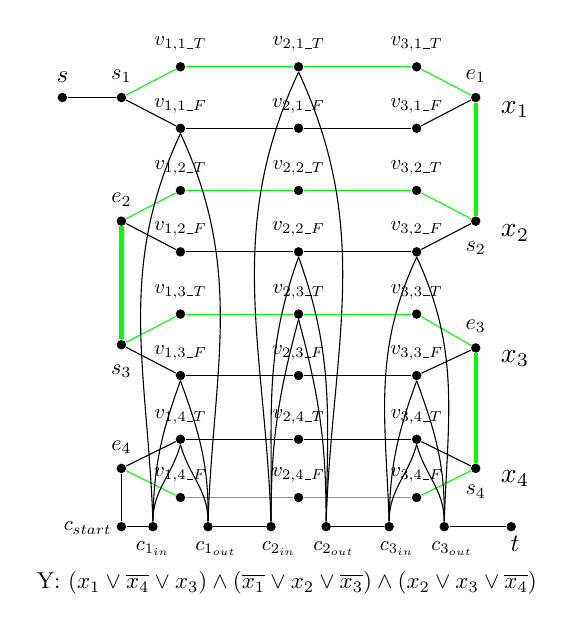
\begin{tikzpicture}[roundnode/.style={circle, fill=black, inner sep=0pt, minimum size=1.2mm}]

    %\foreach \i [count=\ni] in {120,70,...,-180}
        %\node[roundnode] at (\i:1.4cm) (u\ni) {};
    
    \node[roundnode][label=\scalebox{0.9}{${s}$}](u1) at (-1,8.0) {};
    \node[roundnode][label=\scalebox{0.8}{${s_1}$}](u2) at (-0.25,8.0) {};
    \node[roundnode][label=\scalebox{0.75}{${v_{1,1\_T}}$}](u3) at (0.5,8.39) {};
    \node[roundnode][label=\scalebox{0.75}{${v_{1,1\_F}}$}](u4) at (0.5,7.61) {};
    \node[roundnode][label=\scalebox{0.75}{${v_{2,1\_T}}$}](u5) at (2.0,8.39) {};
    \node[roundnode][label=\scalebox{0.75}{${v_{2,1\_F}}$}](u6) at (2.0,7.61) {};
    %\node[roundnode][label=\scalebox{0.75}{${v_{3,1\_T}}$}](u7) at (2.5,8.15) {};
    %\node[roundnode][label=\scalebox{0.75}{${v_{3,1\_F}}$}](u8) at (2.5,7.45) {};
    \node[roundnode][label=\scalebox{0.75}{${v_{3,1\_T}}$}](u9) at (3.5,8.39) {};
    \node[roundnode][label=\scalebox{0.75}{${v_{3,1\_F}}$}](u10) at (3.5,7.61) {};
    \node[roundnode][label=\scalebox{0.8}{$e_1$}](u11) at (4.25,8.0) {};
    \node[style={circle, fill=white, inner sep=0pt, minimum size=0.1mm}][label=\scalebox{1}{$x_1$}](u71) at (4.75, 7.61) {};
    
    \node[roundnode][label=\scalebox{0.8}{${e_2}$}](u12) at (-0.25,6.43) {};
    \node[roundnode][label=\scalebox{0.75}{${v_{1,2\_T}}$}](u13) at (0.5,6.82) {};
    \node[roundnode][label=\scalebox{0.75}{${v_{1,2\_F}}$}](u14) at (0.5,6.04) {};
    \node[roundnode][label=\scalebox{0.75}{${v_{2,2\_T}}$}](u15) at (2.0,6.82) {};
    \node[roundnode][label=\scalebox{0.75}{${v_{2,2\_F}}$}](u16) at (2.0,6.04) {};
    %\node[roundnode][label=\scalebox{0.75}{${v_{3,2\_T}}$}](u17) at (2.5,6.7) {};
    %\node[roundnode][label=\scalebox{0.75}{${v_{3,2\_F}}$}](u18) at (2.5,6) {};
    \node[roundnode][label=\scalebox{0.75}{${v_{3,2\_T}}$}](u19) at (3.5,6.82) {};
    \node[roundnode][label=\scalebox{0.75}{${v_{3,2\_F}}$}](u20) at (3.5,6.04) {};
    \node[roundnode](u21) at (4.25,6.43) {};
    \node[style={circle, fill=white, inner sep=0pt, minimum size=0.2mm}][label=\scalebox{0.8}{$s_2$}](u53) at (4.25, 5.86) {};
    \node[style={circle, fill=white, inner sep=0pt, minimum size=0.1mm}][label=\scalebox{1}{$x_2$}](u72) at (4.75, 6.04) {};
    
    \node[roundnode](u22) at (-0.25,4.86) {};
    \node[style={circle, fill=white, inner sep=0pt, minimum size=0.2mm}][label=\scalebox{0.8}{$s_3$}](u54) at (-0.25, 4.30) {};
    \node[roundnode][label=\scalebox{0.75}{${v_{1,3\_T}}$}](u23) at (0.5,5.25) {};
    \node[roundnode][label=\scalebox{0.75}{${v_{1,3\_F}}$}](u24) at (0.5,4.47) {};
    \node[roundnode][label=\scalebox{0.75}{${v_{2,3\_T}}$}](u25) at (2.0,5.25) {};
    \node[roundnode][label=\scalebox{0.75}{${v_{2,3\_F}}$}](u26) at (2.0,4.47) {};
    %\node[roundnode][label=\scalebox{0.75}{${v_{3,3\_T}}$}](u27) at (2.5,5.25) {};
    %\node[roundnode][label=\scalebox{0.75}{${v_{3,3\_F}}$}](u28) at (2.5,4.55) {};
    \node[roundnode][label=\scalebox{0.75}{${v_{3,3\_T}}$}](u29) at (3.5,5.25) {};
    \node[roundnode][label=\scalebox{0.75}{${v_{3,3\_F}}$}](u30) at (3.5,4.47) {};
    \node[roundnode][label=\scalebox{0.8}{$e_3$}](u31) at (4.25,4.82) {};
    \node[style={circle, fill=white, inner sep=0pt, minimum size=0.1mm}][label=\scalebox{1}{$x_3$}](u73) at (4.75, 4.45) {};
    
    \node[roundnode][label=\scalebox{0.8}{${e_4}$}](u32) at (-0.25,3.29) {};
    \node[roundnode][label=\scalebox{0.75}{${v_{1,4\_T}}$}](u33) at (0.5,3.66) {};
    \node[roundnode][label=\scalebox{0.75}{${v_{1,4\_F}}$}](u34) at (0.5,2.92) {};
    \node[roundnode][label=\scalebox{0.75}{${v_{2,4\_T}}$}](u35) at (2.0,3.66) {};
    \node[roundnode][label=\scalebox{0.75}{${v_{2,4\_F}}$}](u36) at (2.0,2.92) {};
    %\node[roundnode][label=\scalebox{0.75}{${v_{3,4\_T}}$}](u37) at (2.5,3.8) {};
    %\node[roundnode][label=\scalebox{0.75}{${v_{3,4\_F}}$}](u38) at (2.5,3.1) {};
    \node[roundnode][label=\scalebox{0.75}{${v_{3,4\_T}}$}](u39) at (3.5,3.66) {};
    \node[roundnode][label=\scalebox{0.75}{${v_{3,4\_F}}$}](u40) at (3.5,2.92) {};
    \node[roundnode](u41) at (4.25,3.29) {};
    \node[style={circle, fill=white, inner sep=0pt, minimum size=0.2mm}][label=\scalebox{0.8}{$s_4$}](u55) at (4.25, 2.77) {};
    \node[style={circle, fill=white, inner sep=0pt, minimum size=0.1mm}][label=\scalebox{1}{$x_4$}](u74) at (4.75, 2.92) {};
    
    %\node[roundnode](u42) at (-1,3.5) {};
    %\node[roundnode](u43) at (-1,2) {};
    
    \node[roundnode](u43) at (-0.25,2.55) {};
    \node[roundnode](u44) at (0.15,2.55) {};
    \node[roundnode](u45) at (0.85,2.55) {};
    \node[roundnode](u46) at (1.65,2.55) {};
    \node[roundnode](u47) at (2.35,2.55) {};
    %\node[roundnode](u48) at (2.2,2.55) {};
    %\node[roundnode](u49) at (2.8,2.55) {};
    \node[roundnode](u50) at (3.15,2.55) {};
    \node[roundnode](u51) at (3.85,2.55) {};
    
    \node[roundnode](u52) at (4.7,2.55) {};
    \node[style={circle, fill=white, inner sep=0pt, minimum size=0.1mm}][label=\scalebox{0.9}{$t$}](u81) at (4.75, 2.1) {};
    
    \node[style={circle, fill=white, inner sep=0pt, minimum size=0.1mm}][label=\scalebox{0.75}{${c_{1_{in}}}$}](u56) at (0.15,2.05) {};
    \node[style={circle, fill=white, inner sep=0pt, minimum size=0.1mm}][label=\scalebox{0.75}{${c_{1_{out}}}$}](u57) at (0.95,2.05) {};
    \node[style={circle, fill=white, inner sep=0pt, minimum size=0.1mm}][label=\scalebox{0.75}{${c_{2_{in}}}$}](u58) at (1.75,2.05) {};
    \node[style={circle, fill=white, inner sep=0pt, minimum size=0.1mm}][label=\scalebox{0.75}{${c_{2_{out}}}$}](u59) at (2.45,2.05) {};
    \node[style={circle, fill=white, inner sep=0pt, minimum size=0.1mm}][label=\scalebox{0.75}{${c_{3_{in}}}$}](u60) at (3.25,2.05) {};
    \node[style={circle, fill=white, inner sep=0pt, minimum size=0.1mm}][label=\scalebox{0.75}{${c_{3_{out}}}$}](u61) at (3.95,2.05) {};
    
    \node[style={circle, fill=white, inner sep=0pt, minimum size=0.1mm}][label=\scalebox{0.75}{$c_{start}$}](u91) at (-0.68, 2.32) {};
    
            %Lines
            \draw[-] (u1) -- (u2);
            \draw[-, green] (u2) -- (u3);
            \draw[-] (u2) -- (u4);
            \draw[-, green] (u3) -- (u5); 
            \draw[-] (u4) -- (u6);
            %\draw[-] (u5) -- (u7);
            %\draw[-] (u6) -- (u8);
            \draw[-, green] (u5) -- (u9);
            \draw[-] (u6) -- (u10);
            \draw[-, green] (u9) -- (u11); 
            \draw[-] (u10) -- (u11);
            
            \draw[-, ultra thick, green] (u11) -- (u21);
            
            \draw[-, green] (u12) -- (u13);
            \draw[-] (u12) -- (u14);
            \draw[-, green] (u13) -- (u15); 
            \draw[-] (u14) -- (u16);
            %\draw[-] (u15) -- (u17);
            %\draw[-] (u16) -- (u18);
            \draw[-, green] (u15) -- (u19);
            \draw[-] (u16) -- (u20);
            \draw[-, green] (u19) -- (u21); 
            \draw[-] (u20) -- (u21);
            
            \draw[-, ultra thick, green] (u12) -- (u22);
            
            \draw[-, green] (u22) -- (u23);
            \draw[-] (u22) -- (u24);
            \draw[-, green] (u23) -- (u25); 
            \draw[-] (u24) -- (u26);
            %\draw[-] (u25) -- (u27);
            %\draw[-] (u26) -- (u28);
            \draw[-, green] (u25) -- (u29);
            \draw[-] (u26) -- (u30);
            \draw[-, green] (u29) -- (u31); 
            \draw[-] (u30) -- (u31);
            
            \draw[-, ultra thick, green] (u31) -- (u41);
            
            \draw[-] (u32) -- (u33);
            \draw[-, green] (u32) -- (u34);
            \draw[-] (u33) -- (u35); 
            \draw[-, green] (u34) -- (u36);
            %\draw[-] (u35) -- (u37);
            %\draw[-] (u36) -- (u38);
            \draw[-] (u35) -- (u39);
            \draw[-, green] (u36) -- (u40);
            \draw[-] (u39) -- (u41); 
            \draw[-, green] (u40) -- (u41);
            
            %\draw[-] (u32) -- (u42);
            %\draw[-] (u42) -- (u43);
            \draw[-] (u32) -- (u43);
            \draw[-] (u43) -- (u44); 
            \draw[-] (u45) -- (u46);
            %\draw[-] (u47) -- (u48);
            %\draw[-] (u49) -- (u50);
            \draw[-] (u47) -- (u50);
            \draw[-] (u51) -- (u52);
        
            \begin{scope}
                \draw[-] (u4.south) to [out=245,in=92] (u44.north);
                %(u4) -- (u44);
                \draw[-] (u4.south) to [out=295,in=88] (u45.north);
                \draw[-] (u24.south) to [out=250,in=89] (u44.north);
                \draw[-] (u24.south) to [out=290,in=89] (u45.north);
                \draw[-] (u33.south) to [out=255,in=90] (u44.north);
                \draw[-] (u33.south) to [out=285,in=90] (u45.north);
                
                \draw[-] (u5.south) to [out=245,in=92] (u46.north);
                %(u4) -- (u44);
                \draw[-] (u5.south) to [out=295,in=88] (u47.north);
                \draw[-] (u16.south) to [out=250,in=89] (u46.north);
                \draw[-] (u16.south) to [out=290,in=89] (u47.north);
                \draw[-] (u25.south) to [out=255,in=90] (u46.north);
                \draw[-] (u25.south) to [out=285,in=90] (u47.north);
                
                \draw[-] (u20.south) to [out=245,in=92] (u50.north);
                %(u4) -- (u44);
                \draw[-] (u20.south) to [out=295,in=88] (u51.north);
                \draw[-] (u30.south) to [out=250,in=89] (u50.north);
                \draw[-] (u30.south) to [out=290,in=89] (u51.north);
                \draw[-] (u39.south) to [out=255,in=90] (u50.north);
                \draw[-] (u39.south) to [out=285,in=90] (u51.north);
            \end{scope}
        \node[style={circle, fill=white, inner sep=0pt, minimum size=0.1mm}][label=\scalebox{0.83}{Y: $({x_1} \vee \overline{x_4} \vee {x_3}) \wedge (\overline{x_1} \vee{x_2} \vee \overline{x_3}) \wedge
        ({x_2} \vee {x_3} \vee \overline{x_4})$ }](u112) at (1.90, 1.55) {};
            
\end{tikzpicture}}
    \end{overlayarea}
\end{column}
\end{columns}
\end{frame}

\begin{frame}{Reduction from 3-SAT formula}
\setbeamercovered{dynamic}
\begin{columns}
\begin{column}{0.45\textwidth}
\begin{block}{Necessity}
If $Y$ is satisfiable, then $G$ has a path of length of at least $k$.
\end{block}

  \begin{itemize} 
    \item<1->If the term $x_i$ is true
     and clause $c_j$ has the term $x_i$, we take edges from $c_{j_{in}}$ to 
        $x_{i,j\_F}$  % $x_{i,j_F}$ % 
        and from $x_{i,j\_F}$ to $c_{j_{out}}$. And if the term $x_i$ is false and clause $c_j$ has the term $\overline{x_i}$, we need to take edges from $c_{j_{in}}$ to $x_{i,j\_T}$ and from $x_{i,j\_T}$ to $c_{j_{out}}$. 
        \item<2->
        Thus for q clauses, total $2*q$ edges are taken.

\end{itemize}
\end{column}
\begin{column}{0.55\textwidth}
    \begin{overlayarea}{0.55\textwidth}{8cm}
        \only<1->{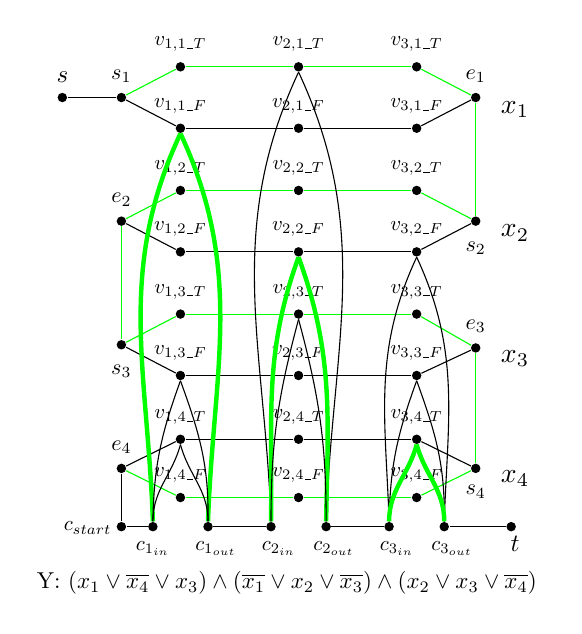
\begin{tikzpicture}[roundnode/.style={circle, fill=black, inner sep=0pt, minimum size=1.2mm}]

    %\foreach \i [count=\ni] in {120,70,...,-180}
        %\node[roundnode] at (\i:1.4cm) (u\ni) {};
    
    \node[roundnode][label=\scalebox{0.9}{${s}$}](u1) at (-1,8.0) {};
    \node[roundnode][label=\scalebox{0.8}{${s_1}$}](u2) at (-0.25,8.0) {};
    \node[roundnode][label=\scalebox{0.75}{${v_{1,1\_T}}$}](u3) at (0.5,8.39) {};
    \node[roundnode][label=\scalebox{0.75}{${v_{1,1\_F}}$}](u4) at (0.5,7.61) {};
    \node[roundnode][label=\scalebox{0.75}{${v_{2,1\_T}}$}](u5) at (2.0,8.39) {};
    \node[roundnode][label=\scalebox{0.75}{${v_{2,1\_F}}$}](u6) at (2.0,7.61) {};
    %\node[roundnode][label=\scalebox{0.75}{${v_{3,1\_T}}$}](u7) at (2.5,8.15) {};
    %\node[roundnode][label=\scalebox{0.75}{${v_{3,1\_F}}$}](u8) at (2.5,7.45) {};
    \node[roundnode][label=\scalebox{0.75}{${v_{3,1\_T}}$}](u9) at (3.5,8.39) {};
    \node[roundnode][label=\scalebox{0.75}{${v_{3,1\_F}}$}](u10) at (3.5,7.61) {};
    \node[roundnode][label=\scalebox{0.8}{$e_1$}](u11) at (4.25,8.0) {};
    \node[style={circle, fill=white, inner sep=0pt, minimum size=0.1mm}][label=\scalebox{1}{$x_1$}](u71) at (4.75, 7.61) {};
    
    \node[roundnode][label=\scalebox{0.8}{${e_2}$}](u12) at (-0.25,6.43) {};
    \node[roundnode][label=\scalebox{0.75}{${v_{1,2\_T}}$}](u13) at (0.5,6.82) {};
    \node[roundnode][label=\scalebox{0.75}{${v_{1,2\_F}}$}](u14) at (0.5,6.04) {};
    \node[roundnode][label=\scalebox{0.75}{${v_{2,2\_T}}$}](u15) at (2.0,6.82) {};
    \node[roundnode][label=\scalebox{0.75}{${v_{2,2\_F}}$}](u16) at (2.0,6.04) {};
    %\node[roundnode][label=\scalebox{0.75}{${v_{3,2\_T}}$}](u17) at (2.5,6.7) {};
    %\node[roundnode][label=\scalebox{0.75}{${v_{3,2\_F}}$}](u18) at (2.5,6) {};
    \node[roundnode][label=\scalebox{0.75}{${v_{3,2\_T}}$}](u19) at (3.5,6.82) {};
    \node[roundnode][label=\scalebox{0.75}{${v_{3,2\_F}}$}](u20) at (3.5,6.04) {};
    \node[roundnode](u21) at (4.25,6.43) {};
    \node[style={circle, fill=white, inner sep=0pt, minimum size=0.2mm}][label=\scalebox{0.8}{$s_2$}](u53) at (4.25, 5.86) {};
    \node[style={circle, fill=white, inner sep=0pt, minimum size=0.1mm}][label=\scalebox{1}{$x_2$}](u72) at (4.75, 6.04) {};
    
    \node[roundnode](u22) at (-0.25,4.86) {};
    \node[style={circle, fill=white, inner sep=0pt, minimum size=0.2mm}][label=\scalebox{0.8}{$s_3$}](u54) at (-0.25, 4.30) {};
    \node[roundnode][label=\scalebox{0.75}{${v_{1,3\_T}}$}](u23) at (0.5,5.25) {};
    \node[roundnode][label=\scalebox{0.75}{${v_{1,3\_F}}$}](u24) at (0.5,4.47) {};
    \node[roundnode][label=\scalebox{0.75}{${v_{2,3\_T}}$}](u25) at (2.0,5.25) {};
    \node[roundnode][label=\scalebox{0.75}{${v_{2,3\_F}}$}](u26) at (2.0,4.47) {};
    %\node[roundnode][label=\scalebox{0.75}{${v_{3,3\_T}}$}](u27) at (2.5,5.25) {};
    %\node[roundnode][label=\scalebox{0.75}{${v_{3,3\_F}}$}](u28) at (2.5,4.55) {};
    \node[roundnode][label=\scalebox{0.75}{${v_{3,3\_T}}$}](u29) at (3.5,5.25) {};
    \node[roundnode][label=\scalebox{0.75}{${v_{3,3\_F}}$}](u30) at (3.5,4.47) {};
    \node[roundnode][label=\scalebox{0.8}{$e_3$}](u31) at (4.25,4.82) {};
    \node[style={circle, fill=white, inner sep=0pt, minimum size=0.1mm}][label=\scalebox{1}{$x_3$}](u73) at (4.75, 4.45) {};
    
    \node[roundnode][label=\scalebox{0.8}{${e_4}$}](u32) at (-0.25,3.29) {};
    \node[roundnode][label=\scalebox{0.75}{${v_{1,4\_T}}$}](u33) at (0.5,3.66) {};
    \node[roundnode][label=\scalebox{0.75}{${v_{1,4\_F}}$}](u34) at (0.5,2.92) {};
    \node[roundnode][label=\scalebox{0.75}{${v_{2,4\_T}}$}](u35) at (2.0,3.66) {};
    \node[roundnode][label=\scalebox{0.75}{${v_{2,4\_F}}$}](u36) at (2.0,2.92) {};
    %\node[roundnode][label=\scalebox{0.75}{${v_{3,4\_T}}$}](u37) at (2.5,3.8) {};
    %\node[roundnode][label=\scalebox{0.75}{${v_{3,4\_F}}$}](u38) at (2.5,3.1) {};
    \node[roundnode][label=\scalebox{0.75}{${v_{3,4\_T}}$}](u39) at (3.5,3.66) {};
    \node[roundnode][label=\scalebox{0.75}{${v_{3,4\_F}}$}](u40) at (3.5,2.92) {};
    \node[roundnode](u41) at (4.25,3.29) {};
    \node[style={circle, fill=white, inner sep=0pt, minimum size=0.2mm}][label=\scalebox{0.8}{$s_4$}](u55) at (4.25, 2.77) {};
    \node[style={circle, fill=white, inner sep=0pt, minimum size=0.1mm}][label=\scalebox{1}{$x_4$}](u74) at (4.75, 2.92) {};
    
    %\node[roundnode](u42) at (-1,3.5) {};
    %\node[roundnode](u43) at (-1,2) {};
    
    \node[roundnode](u43) at (-0.25,2.55) {};
    \node[roundnode](u44) at (0.15,2.55) {};
    \node[roundnode](u45) at (0.85,2.55) {};
    \node[roundnode](u46) at (1.65,2.55) {};
    \node[roundnode](u47) at (2.35,2.55) {};
    %\node[roundnode](u48) at (2.2,2.55) {};
    %\node[roundnode](u49) at (2.8,2.55) {};
    \node[roundnode](u50) at (3.15,2.55) {};
    \node[roundnode](u51) at (3.85,2.55) {};
    
    \node[roundnode](u52) at (4.7,2.55) {};
    \node[style={circle, fill=white, inner sep=0pt, minimum size=0.1mm}][label=\scalebox{0.9}{$t$}](u81) at (4.75, 2.1) {};
    
    \node[style={circle, fill=white, inner sep=0pt, minimum size=0.1mm}][label=\scalebox{0.75}{${c_{1_{in}}}$}](u56) at (0.15,2.05) {};
    \node[style={circle, fill=white, inner sep=0pt, minimum size=0.1mm}][label=\scalebox{0.75}{${c_{1_{out}}}$}](u57) at (0.95,2.05) {};
    \node[style={circle, fill=white, inner sep=0pt, minimum size=0.1mm}][label=\scalebox{0.75}{${c_{2_{in}}}$}](u58) at (1.75,2.05) {};
    \node[style={circle, fill=white, inner sep=0pt, minimum size=0.1mm}][label=\scalebox{0.75}{${c_{2_{out}}}$}](u59) at (2.45,2.05) {};
    \node[style={circle, fill=white, inner sep=0pt, minimum size=0.1mm}][label=\scalebox{0.75}{${c_{3_{in}}}$}](u60) at (3.25,2.05) {};
    \node[style={circle, fill=white, inner sep=0pt, minimum size=0.1mm}][label=\scalebox{0.75}{${c_{3_{out}}}$}](u61) at (3.95,2.05) {};
    
    \node[style={circle, fill=white, inner sep=0pt, minimum size=0.1mm}][label=\scalebox{0.75}{$c_{start}$}](u91) at (-0.68, 2.32) {};
    
            %Lines
            \draw[-] (u1) -- (u2);
            \draw[-, green] (u2) -- (u3);
            \draw[-] (u2) -- (u4);
            \draw[-, green] (u3) -- (u5); 
            \draw[-] (u4) -- (u6);
            %\draw[-] (u5) -- (u7);
            %\draw[-] (u6) -- (u8);
            \draw[-, green] (u5) -- (u9);
            \draw[-] (u6) -- (u10);
            \draw[-, green] (u9) -- (u11); 
            \draw[-] (u10) -- (u11);
            
            \draw[-, green] (u11) -- (u21);
            
            \draw[-, green] (u12) -- (u13);
            \draw[-] (u12) -- (u14);
            \draw[-, green] (u13) -- (u15); 
            \draw[-] (u14) -- (u16);
            %\draw[-] (u15) -- (u17);
            %\draw[-] (u16) -- (u18);
            \draw[-, green] (u15) -- (u19);
            \draw[-] (u16) -- (u20);
            \draw[-, green] (u19) -- (u21); 
            \draw[-] (u20) -- (u21);
            
            \draw[-, green] (u12) -- (u22);
            
            \draw[-, green] (u22) -- (u23);
            \draw[-] (u22) -- (u24);
            \draw[-, green] (u23) -- (u25); 
            \draw[-] (u24) -- (u26);
            %\draw[-] (u25) -- (u27);
            %\draw[-] (u26) -- (u28);
            \draw[-, green] (u25) -- (u29);
            \draw[-] (u26) -- (u30);
            \draw[-, green] (u29) -- (u31); 
            \draw[-] (u30) -- (u31);
            
            \draw[-, green] (u31) -- (u41);
            
            \draw[-] (u32) -- (u33);
            \draw[-, green] (u32) -- (u34);
            \draw[-] (u33) -- (u35); 
            \draw[-, green] (u34) -- (u36);
            %\draw[-] (u35) -- (u37);
            %\draw[-] (u36) -- (u38);
            \draw[-] (u35) -- (u39);
            \draw[-, green] (u36) -- (u40);
            \draw[-] (u39) -- (u41); 
            \draw[-, green] (u40) -- (u41);
            
            %\draw[-] (u32) -- (u42);
            %\draw[-] (u42) -- (u43);
            \draw[-] (u32) -- (u43);
            \draw[-] (u43) -- (u44); 
            \draw[-] (u45) -- (u46);
            %\draw[-] (u47) -- (u48);
            %\draw[-] (u49) -- (u50);
            \draw[-] (u47) -- (u50);
            \draw[-] (u51) -- (u52);
        
            \begin{scope}
                \draw[-, ultra thick, green] (u4.south) to [out=245,in=92] (u44.north);
                %(u4) -- (u44);
                \draw[-, ultra thick, green] (u4.south) to [out=295,in=88] (u45.north);
                \draw[-] (u24.south) to [out=250,in=89] (u44.north);
                \draw[-] (u24.south) to [out=290,in=89] (u45.north);
                \draw[-] (u33.south) to [out=255,in=90] (u44.north);
                \draw[-] (u33.south) to [out=285,in=90] (u45.north);
                
                \draw[-] (u5.south) to [out=245,in=92] (u46.north);
                %(u4) -- (u44);
                \draw[-] (u5.south) to [out=295,in=88] (u47.north);
                \draw[-, ultra thick, green] (u16.south) to [out=250,in=89] (u46.north);
                \draw[-, ultra thick, green] (u16.south) to [out=290,in=89] (u47.north);
                \draw[-] (u25.south) to [out=255,in=90] (u46.north);
                \draw[-] (u25.south) to [out=285,in=90] (u47.north);
                
                \draw[-] (u20.south) to [out=245,in=92] (u50.north);
                %(u4) -- (u44);
                \draw[-] (u20.south) to [out=295,in=88] (u51.north);
                \draw[-] (u30.south) to [out=250,in=89] (u50.north);
                \draw[-] (u30.south) to [out=290,in=89] (u51.north);
                \draw[-, ultra thick, green] (u39.south) to [out=255,in=90] (u50.north);
                \draw[-, ultra thick, green] (u39.south) to [out=285,in=90] (u51.north);
            \end{scope}
        \node[style={circle, fill=white, inner sep=0pt, minimum size=0.1mm}][label=\scalebox{0.83}{Y: $({x_1} \vee \overline{x_4} \vee {x_3}) \wedge (\overline{x_1} \vee{x_2} \vee \overline{x_3}) \wedge
        ({x_2} \vee {x_3} \vee \overline{x_4})$ }](u112) at (1.90, 1.55) {};
        
\end{tikzpicture}}
    \end{overlayarea}
\end{column}
\end{columns}
\end{frame}

\begin{frame}{Reduction from 3-SAT formula}
\setbeamercovered{dynamic}
\begin{columns}
\begin{column}{0.45\textwidth}
\begin{block}{Necessity}
If $Y$ is satisfiable, then $G$ has a path of length of at least $k$.
\end{block}

  \begin{itemize} 
    \item<1->
        To complete the path, edges from $c_{j_{out}}$ to $c_{j+1_{in}}$ must be taken.
        \item<2-> Total $q-1$ edges are taken. 
        \item<3-> Edges from $s$ to $s_1$,
        $e_n$ to $c_{start}$, $c_{start}$ to $c_{1_{in}}$ and $c_{q_{out}}$ to $t$ is taken. 
        \item<4->Thus total $n*(q+1) + n-1 + 2*q + 4$ edges is taken. So the length of the path is $k$.
\end{itemize}
\end{column}
\begin{column}{0.55\textwidth}
    \begin{overlayarea}{0.55\textwidth}{8cm}
        \only<1,2>{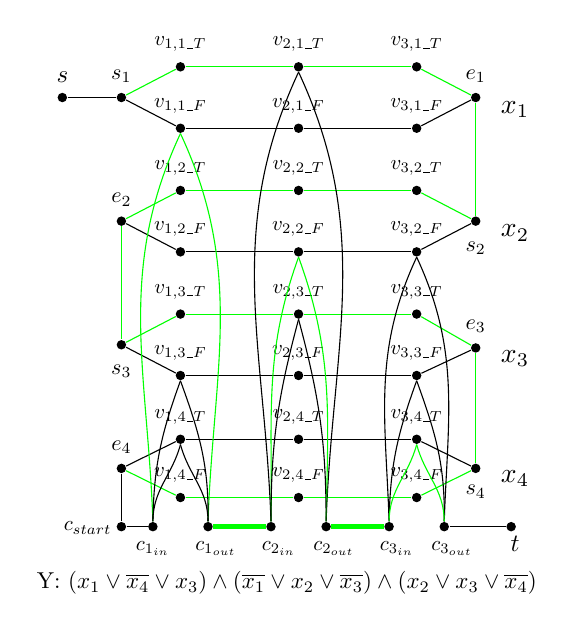
\begin{tikzpicture}[roundnode/.style={circle, fill=black, inner sep=0pt, minimum size=1.2mm}]

    %\foreach \i [count=\ni] in {120,70,...,-180}
        %\node[roundnode] at (\i:1.4cm) (u\ni) {};
    
    \node[roundnode][label=\scalebox{0.9}{${s}$}](u1) at (-1,8.0) {};
    \node[roundnode][label=\scalebox{0.8}{${s_1}$}](u2) at (-0.25,8.0) {};
    \node[roundnode][label=\scalebox{0.75}{${v_{1,1\_T}}$}](u3) at (0.5,8.39) {};
    \node[roundnode][label=\scalebox{0.75}{${v_{1,1\_F}}$}](u4) at (0.5,7.61) {};
    \node[roundnode][label=\scalebox{0.75}{${v_{2,1\_T}}$}](u5) at (2.0,8.39) {};
    \node[roundnode][label=\scalebox{0.75}{${v_{2,1\_F}}$}](u6) at (2.0,7.61) {};
    %\node[roundnode][label=\scalebox{0.75}{${v_{3,1\_T}}$}](u7) at (2.5,8.15) {};
    %\node[roundnode][label=\scalebox{0.75}{${v_{3,1\_F}}$}](u8) at (2.5,7.45) {};
    \node[roundnode][label=\scalebox{0.75}{${v_{3,1\_T}}$}](u9) at (3.5,8.39) {};
    \node[roundnode][label=\scalebox{0.75}{${v_{3,1\_F}}$}](u10) at (3.5,7.61) {};
    \node[roundnode][label=\scalebox{0.8}{$e_1$}](u11) at (4.25,8.0) {};
    \node[style={circle, fill=white, inner sep=0pt, minimum size=0.1mm}][label=\scalebox{1}{$x_1$}](u71) at (4.75, 7.61) {};
    
    \node[roundnode][label=\scalebox{0.8}{${e_2}$}](u12) at (-0.25,6.43) {};
    \node[roundnode][label=\scalebox{0.75}{${v_{1,2\_T}}$}](u13) at (0.5,6.82) {};
    \node[roundnode][label=\scalebox{0.75}{${v_{1,2\_F}}$}](u14) at (0.5,6.04) {};
    \node[roundnode][label=\scalebox{0.75}{${v_{2,2\_T}}$}](u15) at (2.0,6.82) {};
    \node[roundnode][label=\scalebox{0.75}{${v_{2,2\_F}}$}](u16) at (2.0,6.04) {};
    %\node[roundnode][label=\scalebox{0.75}{${v_{3,2\_T}}$}](u17) at (2.5,6.7) {};
    %\node[roundnode][label=\scalebox{0.75}{${v_{3,2\_F}}$}](u18) at (2.5,6) {};
    \node[roundnode][label=\scalebox{0.75}{${v_{3,2\_T}}$}](u19) at (3.5,6.82) {};
    \node[roundnode][label=\scalebox{0.75}{${v_{3,2\_F}}$}](u20) at (3.5,6.04) {};
    \node[roundnode](u21) at (4.25,6.43) {};
    \node[style={circle, fill=white, inner sep=0pt, minimum size=0.2mm}][label=\scalebox{0.8}{$s_2$}](u53) at (4.25, 5.86) {};
    \node[style={circle, fill=white, inner sep=0pt, minimum size=0.1mm}][label=\scalebox{1}{$x_2$}](u72) at (4.75, 6.04) {};
    
    \node[roundnode](u22) at (-0.25,4.86) {};
    \node[style={circle, fill=white, inner sep=0pt, minimum size=0.2mm}][label=\scalebox{0.8}{$s_3$}](u54) at (-0.25, 4.30) {};
    \node[roundnode][label=\scalebox{0.75}{${v_{1,3\_T}}$}](u23) at (0.5,5.25) {};
    \node[roundnode][label=\scalebox{0.75}{${v_{1,3\_F}}$}](u24) at (0.5,4.47) {};
    \node[roundnode][label=\scalebox{0.75}{${v_{2,3\_T}}$}](u25) at (2.0,5.25) {};
    \node[roundnode][label=\scalebox{0.75}{${v_{2,3\_F}}$}](u26) at (2.0,4.47) {};
    %\node[roundnode][label=\scalebox{0.75}{${v_{3,3\_T}}$}](u27) at (2.5,5.25) {};
    %\node[roundnode][label=\scalebox{0.75}{${v_{3,3\_F}}$}](u28) at (2.5,4.55) {};
    \node[roundnode][label=\scalebox{0.75}{${v_{3,3\_T}}$}](u29) at (3.5,5.25) {};
    \node[roundnode][label=\scalebox{0.75}{${v_{3,3\_F}}$}](u30) at (3.5,4.47) {};
    \node[roundnode][label=\scalebox{0.8}{$e_3$}](u31) at (4.25,4.82) {};
    \node[style={circle, fill=white, inner sep=0pt, minimum size=0.1mm}][label=\scalebox{1}{$x_3$}](u73) at (4.75, 4.45) {};
    
    \node[roundnode][label=\scalebox{0.8}{${e_4}$}](u32) at (-0.25,3.29) {};
    \node[roundnode][label=\scalebox{0.75}{${v_{1,4\_T}}$}](u33) at (0.5,3.66) {};
    \node[roundnode][label=\scalebox{0.75}{${v_{1,4\_F}}$}](u34) at (0.5,2.92) {};
    \node[roundnode][label=\scalebox{0.75}{${v_{2,4\_T}}$}](u35) at (2.0,3.66) {};
    \node[roundnode][label=\scalebox{0.75}{${v_{2,4\_F}}$}](u36) at (2.0,2.92) {};
    %\node[roundnode][label=\scalebox{0.75}{${v_{3,4\_T}}$}](u37) at (2.5,3.8) {};
    %\node[roundnode][label=\scalebox{0.75}{${v_{3,4\_F}}$}](u38) at (2.5,3.1) {};
    \node[roundnode][label=\scalebox{0.75}{${v_{3,4\_T}}$}](u39) at (3.5,3.66) {};
    \node[roundnode][label=\scalebox{0.75}{${v_{3,4\_F}}$}](u40) at (3.5,2.92) {};
    \node[roundnode](u41) at (4.25,3.29) {};
    \node[style={circle, fill=white, inner sep=0pt, minimum size=0.2mm}][label=\scalebox{0.8}{$s_4$}](u55) at (4.25, 2.77) {};
    \node[style={circle, fill=white, inner sep=0pt, minimum size=0.1mm}][label=\scalebox{1}{$x_4$}](u74) at (4.75, 2.92) {};
    
    %\node[roundnode](u42) at (-1,3.5) {};
    %\node[roundnode](u43) at (-1,2) {};
    
    \node[roundnode](u43) at (-0.25,2.55) {};
    \node[roundnode](u44) at (0.15,2.55) {};
    \node[roundnode](u45) at (0.85,2.55) {};
    \node[roundnode](u46) at (1.65,2.55) {};
    \node[roundnode](u47) at (2.35,2.55) {};
    %\node[roundnode](u48) at (2.2,2.55) {};
    %\node[roundnode](u49) at (2.8,2.55) {};
    \node[roundnode](u50) at (3.15,2.55) {};
    \node[roundnode](u51) at (3.85,2.55) {};
    
    \node[roundnode](u52) at (4.7,2.55) {};
    \node[style={circle, fill=white, inner sep=0pt, minimum size=0.1mm}][label=\scalebox{0.9}{$t$}](u81) at (4.75, 2.1) {};
    
    \node[style={circle, fill=white, inner sep=0pt, minimum size=0.1mm}][label=\scalebox{0.75}{${c_{1_{in}}}$}](u56) at (0.15,2.05) {};
    \node[style={circle, fill=white, inner sep=0pt, minimum size=0.1mm}][label=\scalebox{0.75}{${c_{1_{out}}}$}](u57) at (0.95,2.05) {};
    \node[style={circle, fill=white, inner sep=0pt, minimum size=0.1mm}][label=\scalebox{0.75}{${c_{2_{in}}}$}](u58) at (1.75,2.05) {};
    \node[style={circle, fill=white, inner sep=0pt, minimum size=0.1mm}][label=\scalebox{0.75}{${c_{2_{out}}}$}](u59) at (2.45,2.05) {};
    \node[style={circle, fill=white, inner sep=0pt, minimum size=0.1mm}][label=\scalebox{0.75}{${c_{3_{in}}}$}](u60) at (3.25,2.05) {};
    \node[style={circle, fill=white, inner sep=0pt, minimum size=0.1mm}][label=\scalebox{0.75}{${c_{3_{out}}}$}](u61) at (3.95,2.05) {};
    
    \node[style={circle, fill=white, inner sep=0pt, minimum size=0.1mm}][label=\scalebox{0.75}{$c_{start}$}](u91) at (-0.68, 2.32) {};
    
            %Lines
            \draw[-] (u1) -- (u2);
            \draw[-, green] (u2) -- (u3);
            \draw[-] (u2) -- (u4);
            \draw[-, green] (u3) -- (u5); 
            \draw[-] (u4) -- (u6);
            %\draw[-] (u5) -- (u7);
            %\draw[-] (u6) -- (u8);
            \draw[-, green] (u5) -- (u9);
            \draw[-] (u6) -- (u10);
            \draw[-, green] (u9) -- (u11); 
            \draw[-] (u10) -- (u11);
            
            \draw[-, green] (u11) -- (u21);
            
            \draw[-, green] (u12) -- (u13);
            \draw[-] (u12) -- (u14);
            \draw[-, green] (u13) -- (u15); 
            \draw[-] (u14) -- (u16);
            %\draw[-] (u15) -- (u17);
            %\draw[-] (u16) -- (u18);
            \draw[-, green] (u15) -- (u19);
            \draw[-] (u16) -- (u20);
            \draw[-, green] (u19) -- (u21); 
            \draw[-] (u20) -- (u21);
            
            \draw[-, green] (u12) -- (u22);
            
            \draw[-, green] (u22) -- (u23);
            \draw[-] (u22) -- (u24);
            \draw[-, green] (u23) -- (u25); 
            \draw[-] (u24) -- (u26);
            %\draw[-] (u25) -- (u27);
            %\draw[-] (u26) -- (u28);
            \draw[-, green] (u25) -- (u29);
            \draw[-] (u26) -- (u30);
            \draw[-, green] (u29) -- (u31); 
            \draw[-] (u30) -- (u31);
            
            \draw[-, green] (u31) -- (u41);
            
            \draw[-] (u32) -- (u33);
            \draw[-, green] (u32) -- (u34);
            \draw[-] (u33) -- (u35); 
            \draw[-, green] (u34) -- (u36);
            %\draw[-] (u35) -- (u37);
            %\draw[-] (u36) -- (u38);
            \draw[-] (u35) -- (u39);
            \draw[-, green] (u36) -- (u40);
            \draw[-] (u39) -- (u41); 
            \draw[-, green] (u40) -- (u41);
            
            %\draw[-] (u32) -- (u42);
            %\draw[-] (u42) -- (u43);
            \draw[-] (u32) -- (u43);
            \draw[-] (u43) -- (u44); 
            \draw[-, ultra thick, green] (u45) -- (u46);
            %\draw[-] (u47) -- (u48);
            %\draw[-] (u49) -- (u50);
            \draw[-, ultra thick, green] (u47) -- (u50);
            \draw[-] (u51) -- (u52);
        
            \begin{scope}
                \draw[-, green] (u4.south) to [out=245,in=92] (u44.north);
                %(u4) -- (u44);
                \draw[-, green] (u4.south) to [out=295,in=88] (u45.north);
                \draw[-] (u24.south) to [out=250,in=89] (u44.north);
                \draw[-] (u24.south) to [out=290,in=89] (u45.north);
                \draw[-] (u33.south) to [out=255,in=90] (u44.north);
                \draw[-] (u33.south) to [out=285,in=90] (u45.north);
                
                \draw[-] (u5.south) to [out=245,in=92] (u46.north);
                %(u4) -- (u44);
                \draw[-] (u5.south) to [out=295,in=88] (u47.north);
                \draw[-, green] (u16.south) to [out=250,in=89] (u46.north);
                \draw[-, green] (u16.south) to [out=290,in=89] (u47.north);
                \draw[-] (u25.south) to [out=255,in=90] (u46.north);
                \draw[-] (u25.south) to [out=285,in=90] (u47.north);
                
                \draw[-] (u20.south) to [out=245,in=92] (u50.north);
                %(u4) -- (u44);
                \draw[-] (u20.south) to [out=295,in=88] (u51.north);
                \draw[-] (u30.south) to [out=250,in=89] (u50.north);
                \draw[-] (u30.south) to [out=290,in=89] (u51.north);
                \draw[-, green] (u39.south) to [out=255,in=90] (u50.north);
                \draw[-, green] (u39.south) to [out=285,in=90] (u51.north);
            \end{scope}
        \node[style={circle, fill=white, inner sep=0pt, minimum size=0.1mm}][label=\scalebox{0.83}{Y: $({x_1} \vee \overline{x_4} \vee {x_3}) \wedge (\overline{x_1} \vee{x_2} \vee \overline{x_3}) \wedge
        ({x_2} \vee {x_3} \vee \overline{x_4})$ }](u112) at (1.90, 1.55) {};
        
\end{tikzpicture}}
        \only<3>{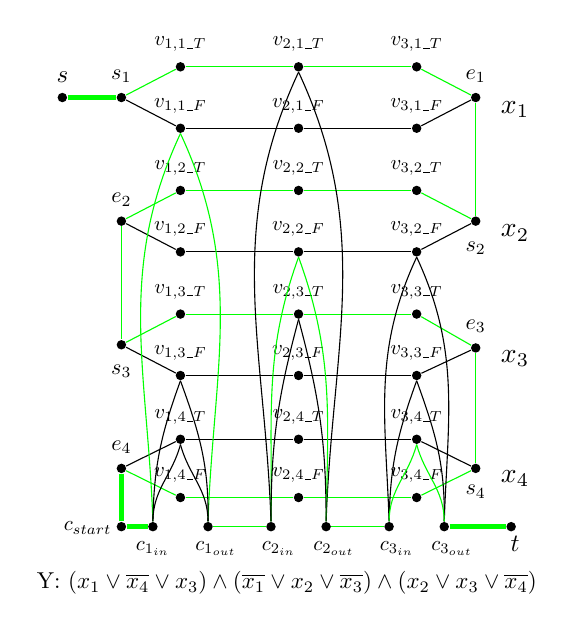
\begin{tikzpicture}[roundnode/.style={circle, fill=black, inner sep=0pt, minimum size=1.2mm}]

    %\foreach \i [count=\ni] in {120,70,...,-180}
        %\node[roundnode] at (\i:1.4cm) (u\ni) {};
    
    \node[roundnode][label=\scalebox{0.9}{${s}$}](u1) at (-1,8.0) {};
    \node[roundnode][label=\scalebox{0.8}{${s_1}$}](u2) at (-0.25,8.0) {};
    \node[roundnode][label=\scalebox{0.75}{${v_{1,1\_T}}$}](u3) at (0.5,8.39) {};
    \node[roundnode][label=\scalebox{0.75}{${v_{1,1\_F}}$}](u4) at (0.5,7.61) {};
    \node[roundnode][label=\scalebox{0.75}{${v_{2,1\_T}}$}](u5) at (2.0,8.39) {};
    \node[roundnode][label=\scalebox{0.75}{${v_{2,1\_F}}$}](u6) at (2.0,7.61) {};
    %\node[roundnode][label=\scalebox{0.75}{${v_{3,1\_T}}$}](u7) at (2.5,8.15) {};
    %\node[roundnode][label=\scalebox{0.75}{${v_{3,1\_F}}$}](u8) at (2.5,7.45) {};
    \node[roundnode][label=\scalebox{0.75}{${v_{3,1\_T}}$}](u9) at (3.5,8.39) {};
    \node[roundnode][label=\scalebox{0.75}{${v_{3,1\_F}}$}](u10) at (3.5,7.61) {};
    \node[roundnode][label=\scalebox{0.8}{$e_1$}](u11) at (4.25,8.0) {};
    \node[style={circle, fill=white, inner sep=0pt, minimum size=0.1mm}][label=\scalebox{1}{$x_1$}](u71) at (4.75, 7.61) {};
    
    \node[roundnode][label=\scalebox{0.8}{${e_2}$}](u12) at (-0.25,6.43) {};
    \node[roundnode][label=\scalebox{0.75}{${v_{1,2\_T}}$}](u13) at (0.5,6.82) {};
    \node[roundnode][label=\scalebox{0.75}{${v_{1,2\_F}}$}](u14) at (0.5,6.04) {};
    \node[roundnode][label=\scalebox{0.75}{${v_{2,2\_T}}$}](u15) at (2.0,6.82) {};
    \node[roundnode][label=\scalebox{0.75}{${v_{2,2\_F}}$}](u16) at (2.0,6.04) {};
    %\node[roundnode][label=\scalebox{0.75}{${v_{3,2\_T}}$}](u17) at (2.5,6.7) {};
    %\node[roundnode][label=\scalebox{0.75}{${v_{3,2\_F}}$}](u18) at (2.5,6) {};
    \node[roundnode][label=\scalebox{0.75}{${v_{3,2\_T}}$}](u19) at (3.5,6.82) {};
    \node[roundnode][label=\scalebox{0.75}{${v_{3,2\_F}}$}](u20) at (3.5,6.04) {};
    \node[roundnode](u21) at (4.25,6.43) {};
    \node[style={circle, fill=white, inner sep=0pt, minimum size=0.2mm}][label=\scalebox{0.8}{$s_2$}](u53) at (4.25, 5.86) {};
    \node[style={circle, fill=white, inner sep=0pt, minimum size=0.1mm}][label=\scalebox{1}{$x_2$}](u72) at (4.75, 6.04) {};
    
    \node[roundnode](u22) at (-0.25,4.86) {};
    \node[style={circle, fill=white, inner sep=0pt, minimum size=0.2mm}][label=\scalebox{0.8}{$s_3$}](u54) at (-0.25, 4.30) {};
    \node[roundnode][label=\scalebox{0.75}{${v_{1,3\_T}}$}](u23) at (0.5,5.25) {};
    \node[roundnode][label=\scalebox{0.75}{${v_{1,3\_F}}$}](u24) at (0.5,4.47) {};
    \node[roundnode][label=\scalebox{0.75}{${v_{2,3\_T}}$}](u25) at (2.0,5.25) {};
    \node[roundnode][label=\scalebox{0.75}{${v_{2,3\_F}}$}](u26) at (2.0,4.47) {};
    %\node[roundnode][label=\scalebox{0.75}{${v_{3,3\_T}}$}](u27) at (2.5,5.25) {};
    %\node[roundnode][label=\scalebox{0.75}{${v_{3,3\_F}}$}](u28) at (2.5,4.55) {};
    \node[roundnode][label=\scalebox{0.75}{${v_{3,3\_T}}$}](u29) at (3.5,5.25) {};
    \node[roundnode][label=\scalebox{0.75}{${v_{3,3\_F}}$}](u30) at (3.5,4.47) {};
    \node[roundnode][label=\scalebox{0.8}{$e_3$}](u31) at (4.25,4.82) {};
    \node[style={circle, fill=white, inner sep=0pt, minimum size=0.1mm}][label=\scalebox{1}{$x_3$}](u73) at (4.75, 4.45) {};
    
    \node[roundnode][label=\scalebox{0.8}{${e_4}$}](u32) at (-0.25,3.29) {};
    \node[roundnode][label=\scalebox{0.75}{${v_{1,4\_T}}$}](u33) at (0.5,3.66) {};
    \node[roundnode][label=\scalebox{0.75}{${v_{1,4\_F}}$}](u34) at (0.5,2.92) {};
    \node[roundnode][label=\scalebox{0.75}{${v_{2,4\_T}}$}](u35) at (2.0,3.66) {};
    \node[roundnode][label=\scalebox{0.75}{${v_{2,4\_F}}$}](u36) at (2.0,2.92) {};
    %\node[roundnode][label=\scalebox{0.75}{${v_{3,4\_T}}$}](u37) at (2.5,3.8) {};
    %\node[roundnode][label=\scalebox{0.75}{${v_{3,4\_F}}$}](u38) at (2.5,3.1) {};
    \node[roundnode][label=\scalebox{0.75}{${v_{3,4\_T}}$}](u39) at (3.5,3.66) {};
    \node[roundnode][label=\scalebox{0.75}{${v_{3,4\_F}}$}](u40) at (3.5,2.92) {};
    \node[roundnode](u41) at (4.25,3.29) {};
    \node[style={circle, fill=white, inner sep=0pt, minimum size=0.2mm}][label=\scalebox{0.8}{$s_4$}](u55) at (4.25, 2.77) {};
    \node[style={circle, fill=white, inner sep=0pt, minimum size=0.1mm}][label=\scalebox{1}{$x_4$}](u74) at (4.75, 2.92) {};
    
    %\node[roundnode](u42) at (-1,3.5) {};
    %\node[roundnode](u43) at (-1,2) {};
    
    \node[roundnode](u43) at (-0.25,2.55) {};
    \node[roundnode](u44) at (0.15,2.55) {};
    \node[roundnode](u45) at (0.85,2.55) {};
    \node[roundnode](u46) at (1.65,2.55) {};
    \node[roundnode](u47) at (2.35,2.55) {};
    %\node[roundnode](u48) at (2.2,2.55) {};
    %\node[roundnode](u49) at (2.8,2.55) {};
    \node[roundnode](u50) at (3.15,2.55) {};
    \node[roundnode](u51) at (3.85,2.55) {};
    
    \node[roundnode](u52) at (4.7,2.55) {};
    \node[style={circle, fill=white, inner sep=0pt, minimum size=0.1mm}][label=\scalebox{0.9}{$t$}](u81) at (4.75, 2.1) {};
    
    \node[style={circle, fill=white, inner sep=0pt, minimum size=0.1mm}][label=\scalebox{0.75}{${c_{1_{in}}}$}](u56) at (0.15,2.05) {};
    \node[style={circle, fill=white, inner sep=0pt, minimum size=0.1mm}][label=\scalebox{0.75}{${c_{1_{out}}}$}](u57) at (0.95,2.05) {};
    \node[style={circle, fill=white, inner sep=0pt, minimum size=0.1mm}][label=\scalebox{0.75}{${c_{2_{in}}}$}](u58) at (1.75,2.05) {};
    \node[style={circle, fill=white, inner sep=0pt, minimum size=0.1mm}][label=\scalebox{0.75}{${c_{2_{out}}}$}](u59) at (2.45,2.05) {};
    \node[style={circle, fill=white, inner sep=0pt, minimum size=0.1mm}][label=\scalebox{0.75}{${c_{3_{in}}}$}](u60) at (3.25,2.05) {};
    \node[style={circle, fill=white, inner sep=0pt, minimum size=0.1mm}][label=\scalebox{0.75}{${c_{3_{out}}}$}](u61) at (3.95,2.05) {};
    
    \node[style={circle, fill=white, inner sep=0pt, minimum size=0.1mm}][label=\scalebox{0.75}{$c_{start}$}](u91) at (-0.68, 2.32) {};
    
            %Lines
            \draw[-, ultra thick, green] (u1) -- (u2);
            \draw[-, green] (u2) -- (u3);
            \draw[-] (u2) -- (u4);
            \draw[-, green] (u3) -- (u5); 
            \draw[-] (u4) -- (u6);
            %\draw[-] (u5) -- (u7);
            %\draw[-] (u6) -- (u8);
            \draw[-, green] (u5) -- (u9);
            \draw[-] (u6) -- (u10);
            \draw[-, green] (u9) -- (u11); 
            \draw[-] (u10) -- (u11);
            
            \draw[-, green] (u11) -- (u21);
            
            \draw[-, green] (u12) -- (u13);
            \draw[-] (u12) -- (u14);
            \draw[-, green] (u13) -- (u15); 
            \draw[-] (u14) -- (u16);
            %\draw[-] (u15) -- (u17);
            %\draw[-] (u16) -- (u18);
            \draw[-, green] (u15) -- (u19);
            \draw[-] (u16) -- (u20);
            \draw[-, green] (u19) -- (u21); 
            \draw[-] (u20) -- (u21);
            
            \draw[-, green] (u12) -- (u22);
            
            \draw[-, green] (u22) -- (u23);
            \draw[-] (u22) -- (u24);
            \draw[-, green] (u23) -- (u25); 
            \draw[-] (u24) -- (u26);
            %\draw[-] (u25) -- (u27);
            %\draw[-] (u26) -- (u28);
            \draw[-, green] (u25) -- (u29);
            \draw[-] (u26) -- (u30);
            \draw[-, green] (u29) -- (u31); 
            \draw[-] (u30) -- (u31);
            
            \draw[-, green] (u31) -- (u41);
            
            \draw[-] (u32) -- (u33);
            \draw[-, green] (u32) -- (u34);
            \draw[-] (u33) -- (u35); 
            \draw[-, green] (u34) -- (u36);
            %\draw[-] (u35) -- (u37);
            %\draw[-] (u36) -- (u38);
            \draw[-] (u35) -- (u39);
            \draw[-, green] (u36) -- (u40);
            \draw[-] (u39) -- (u41); 
            \draw[-, green] (u40) -- (u41);
            
            %\draw[-] (u32) -- (u42);
            %\draw[-] (u42) -- (u43);
            \draw[-, ultra thick, green] (u32) -- (u43);
            \draw[-, ultra thick, green] (u43) -- (u44); 
            \draw[-, green] (u45) -- (u46);
            %\draw[-] (u47) -- (u48);
            %\draw[-] (u49) -- (u50);
            \draw[-, green] (u47) -- (u50);
            \draw[-, ultra thick, green] (u51) -- (u52);
        
            \begin{scope}
                \draw[-, green] (u4.south) to [out=245,in=92] (u44.north);
                %(u4) -- (u44);
                \draw[-, green] (u4.south) to [out=295,in=88] (u45.north);
                \draw[-] (u24.south) to [out=250,in=89] (u44.north);
                \draw[-] (u24.south) to [out=290,in=89] (u45.north);
                \draw[-] (u33.south) to [out=255,in=90] (u44.north);
                \draw[-] (u33.south) to [out=285,in=90] (u45.north);
                
                \draw[-] (u5.south) to [out=245,in=92] (u46.north);
                %(u4) -- (u44);
                \draw[-] (u5.south) to [out=295,in=88] (u47.north);
                \draw[-, green] (u16.south) to [out=250,in=89] (u46.north);
                \draw[-, green] (u16.south) to [out=290,in=89] (u47.north);
                \draw[-] (u25.south) to [out=255,in=90] (u46.north);
                \draw[-] (u25.south) to [out=285,in=90] (u47.north);
                
                \draw[-] (u20.south) to [out=245,in=92] (u50.north);
                %(u4) -- (u44);
                \draw[-] (u20.south) to [out=295,in=88] (u51.north);
                \draw[-] (u30.south) to [out=250,in=89] (u50.north);
                \draw[-] (u30.south) to [out=290,in=89] (u51.north);
                \draw[-, green] (u39.south) to [out=255,in=90] (u50.north);
                \draw[-, green] (u39.south) to [out=285,in=90] (u51.north);
            \end{scope}
        \node[style={circle, fill=white, inner sep=0pt, minimum size=0.1mm}][label=\scalebox{0.83}{Y: $({x_1} \vee \overline{x_4} \vee {x_3}) \wedge (\overline{x_1} \vee{x_2} \vee \overline{x_3}) \wedge
        ({x_2} \vee {x_3} \vee \overline{x_4})$ }](u112) at (1.90, 1.55) {};
        
\end{tikzpicture}}
        \only<4>{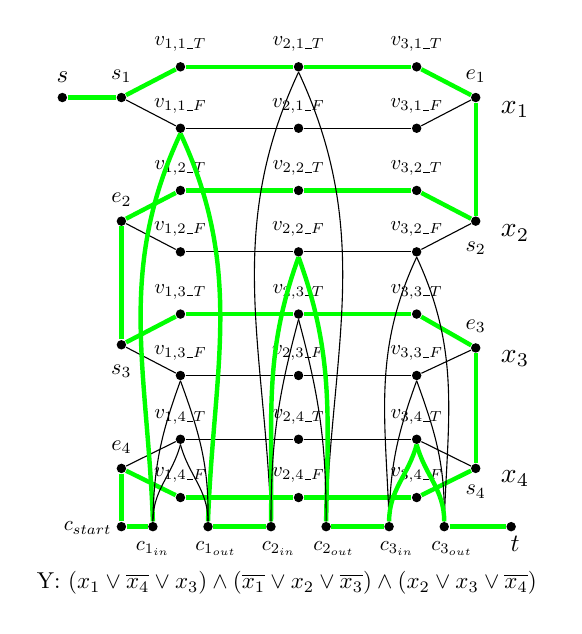
\begin{tikzpicture}[roundnode/.style={circle, fill=black, inner sep=0pt, minimum size=1.2mm}]

    %\foreach \i [count=\ni] in {120,70,...,-180}
        %\node[roundnode] at (\i:1.4cm) (u\ni) {};
    
    \node[roundnode][label=\scalebox{0.9}{${s}$}](u1) at (-1,8.0) {};
    \node[roundnode][label=\scalebox{0.8}{${s_1}$}](u2) at (-0.25,8.0) {};
    \node[roundnode][label=\scalebox{0.75}{${v_{1,1\_T}}$}](u3) at (0.5,8.39) {};
    \node[roundnode][label=\scalebox{0.75}{${v_{1,1\_F}}$}](u4) at (0.5,7.61) {};
    \node[roundnode][label=\scalebox{0.75}{${v_{2,1\_T}}$}](u5) at (2.0,8.39) {};
    \node[roundnode][label=\scalebox{0.75}{${v_{2,1\_F}}$}](u6) at (2.0,7.61) {};
    %\node[roundnode][label=\scalebox{0.75}{${v_{3,1\_T}}$}](u7) at (2.5,8.15) {};
    %\node[roundnode][label=\scalebox{0.75}{${v_{3,1\_F}}$}](u8) at (2.5,7.45) {};
    \node[roundnode][label=\scalebox{0.75}{${v_{3,1\_T}}$}](u9) at (3.5,8.39) {};
    \node[roundnode][label=\scalebox{0.75}{${v_{3,1\_F}}$}](u10) at (3.5,7.61) {};
    \node[roundnode][label=\scalebox{0.8}{$e_1$}](u11) at (4.25,8.0) {};
    \node[style={circle, fill=white, inner sep=0pt, minimum size=0.1mm}][label=\scalebox{1}{$x_1$}](u71) at (4.75, 7.61) {};
    
    \node[roundnode][label=\scalebox{0.8}{${e_2}$}](u12) at (-0.25,6.43) {};
    \node[roundnode][label=\scalebox{0.75}{${v_{1,2\_T}}$}](u13) at (0.5,6.82) {};
    \node[roundnode][label=\scalebox{0.75}{${v_{1,2\_F}}$}](u14) at (0.5,6.04) {};
    \node[roundnode][label=\scalebox{0.75}{${v_{2,2\_T}}$}](u15) at (2.0,6.82) {};
    \node[roundnode][label=\scalebox{0.75}{${v_{2,2\_F}}$}](u16) at (2.0,6.04) {};
    %\node[roundnode][label=\scalebox{0.75}{${v_{3,2\_T}}$}](u17) at (2.5,6.7) {};
    %\node[roundnode][label=\scalebox{0.75}{${v_{3,2\_F}}$}](u18) at (2.5,6) {};
    \node[roundnode][label=\scalebox{0.75}{${v_{3,2\_T}}$}](u19) at (3.5,6.82) {};
    \node[roundnode][label=\scalebox{0.75}{${v_{3,2\_F}}$}](u20) at (3.5,6.04) {};
    \node[roundnode](u21) at (4.25,6.43) {};
    \node[style={circle, fill=white, inner sep=0pt, minimum size=0.2mm}][label=\scalebox{0.8}{$s_2$}](u53) at (4.25, 5.86) {};
    \node[style={circle, fill=white, inner sep=0pt, minimum size=0.1mm}][label=\scalebox{1}{$x_2$}](u72) at (4.75, 6.04) {};
    
    \node[roundnode](u22) at (-0.25,4.86) {};
    \node[style={circle, fill=white, inner sep=0pt, minimum size=0.2mm}][label=\scalebox{0.8}{$s_3$}](u54) at (-0.25, 4.30) {};
    \node[roundnode][label=\scalebox{0.75}{${v_{1,3\_T}}$}](u23) at (0.5,5.25) {};
    \node[roundnode][label=\scalebox{0.75}{${v_{1,3\_F}}$}](u24) at (0.5,4.47) {};
    \node[roundnode][label=\scalebox{0.75}{${v_{2,3\_T}}$}](u25) at (2.0,5.25) {};
    \node[roundnode][label=\scalebox{0.75}{${v_{2,3\_F}}$}](u26) at (2.0,4.47) {};
    %\node[roundnode][label=\scalebox{0.75}{${v_{3,3\_T}}$}](u27) at (2.5,5.25) {};
    %\node[roundnode][label=\scalebox{0.75}{${v_{3,3\_F}}$}](u28) at (2.5,4.55) {};
    \node[roundnode][label=\scalebox{0.75}{${v_{3,3\_T}}$}](u29) at (3.5,5.25) {};
    \node[roundnode][label=\scalebox{0.75}{${v_{3,3\_F}}$}](u30) at (3.5,4.47) {};
    \node[roundnode][label=\scalebox{0.8}{$e_3$}](u31) at (4.25,4.82) {};
    \node[style={circle, fill=white, inner sep=0pt, minimum size=0.1mm}][label=\scalebox{1}{$x_3$}](u73) at (4.75, 4.45) {};
    
    \node[roundnode][label=\scalebox{0.8}{${e_4}$}](u32) at (-0.25,3.29) {};
    \node[roundnode][label=\scalebox{0.75}{${v_{1,4\_T}}$}](u33) at (0.5,3.66) {};
    \node[roundnode][label=\scalebox{0.75}{${v_{1,4\_F}}$}](u34) at (0.5,2.92) {};
    \node[roundnode][label=\scalebox{0.75}{${v_{2,4\_T}}$}](u35) at (2.0,3.66) {};
    \node[roundnode][label=\scalebox{0.75}{${v_{2,4\_F}}$}](u36) at (2.0,2.92) {};
    %\node[roundnode][label=\scalebox{0.75}{${v_{3,4\_T}}$}](u37) at (2.5,3.8) {};
    %\node[roundnode][label=\scalebox{0.75}{${v_{3,4\_F}}$}](u38) at (2.5,3.1) {};
    \node[roundnode][label=\scalebox{0.75}{${v_{3,4\_T}}$}](u39) at (3.5,3.66) {};
    \node[roundnode][label=\scalebox{0.75}{${v_{3,4\_F}}$}](u40) at (3.5,2.92) {};
    \node[roundnode](u41) at (4.25,3.29) {};
    \node[style={circle, fill=white, inner sep=0pt, minimum size=0.2mm}][label=\scalebox{0.8}{$s_4$}](u55) at (4.25, 2.77) {};
    \node[style={circle, fill=white, inner sep=0pt, minimum size=0.1mm}][label=\scalebox{1}{$x_4$}](u74) at (4.75, 2.92) {};
    
    %\node[roundnode](u42) at (-1,3.5) {};
    %\node[roundnode](u43) at (-1,2) {};
    
    \node[roundnode](u43) at (-0.25,2.55) {};
    \node[roundnode](u44) at (0.15,2.55) {};
    \node[roundnode](u45) at (0.85,2.55) {};
    \node[roundnode](u46) at (1.65,2.55) {};
    \node[roundnode](u47) at (2.35,2.55) {};
    %\node[roundnode](u48) at (2.2,2.55) {};
    %\node[roundnode](u49) at (2.8,2.55) {};
    \node[roundnode](u50) at (3.15,2.55) {};
    \node[roundnode](u51) at (3.85,2.55) {};
    
    \node[roundnode](u52) at (4.7,2.55) {};
    \node[style={circle, fill=white, inner sep=0pt, minimum size=0.1mm}][label=\scalebox{0.9}{$t$}](u81) at (4.75, 2.1) {};
    
    \node[style={circle, fill=white, inner sep=0pt, minimum size=0.1mm}][label=\scalebox{0.75}{${c_{1_{in}}}$}](u56) at (0.15,2.05) {};
    \node[style={circle, fill=white, inner sep=0pt, minimum size=0.1mm}][label=\scalebox{0.75}{${c_{1_{out}}}$}](u57) at (0.95,2.05) {};
    \node[style={circle, fill=white, inner sep=0pt, minimum size=0.1mm}][label=\scalebox{0.75}{${c_{2_{in}}}$}](u58) at (1.75,2.05) {};
    \node[style={circle, fill=white, inner sep=0pt, minimum size=0.1mm}][label=\scalebox{0.75}{${c_{2_{out}}}$}](u59) at (2.45,2.05) {};
    \node[style={circle, fill=white, inner sep=0pt, minimum size=0.1mm}][label=\scalebox{0.75}{${c_{3_{in}}}$}](u60) at (3.25,2.05) {};
    \node[style={circle, fill=white, inner sep=0pt, minimum size=0.1mm}][label=\scalebox{0.75}{${c_{3_{out}}}$}](u61) at (3.95,2.05) {};
    
    \node[style={circle, fill=white, inner sep=0pt, minimum size=0.1mm}][label=\scalebox{0.75}{$c_{start}$}](u91) at (-0.68, 2.32) {};
    
            %Lines
            \draw[-, ultra thick, green] (u1) -- (u2);
            \draw[-, ultra thick, green] (u2) -- (u3);
            \draw[-] (u2) -- (u4);
            \draw[-, ultra thick, green] (u3) -- (u5); 
            \draw[-] (u4) -- (u6);
            %\draw[-] (u5) -- (u7);
            %\draw[-] (u6) -- (u8);
            \draw[-, ultra thick, green] (u5) -- (u9);
            \draw[-] (u6) -- (u10);
            \draw[-, ultra thick, green] (u9) -- (u11); 
            \draw[-] (u10) -- (u11);
            
            \draw[-, ultra thick, green] (u11) -- (u21);
            
            \draw[-, ultra thick, green] (u12) -- (u13);
            \draw[-] (u12) -- (u14);
            \draw[-, ultra thick, green] (u13) -- (u15); 
            \draw[-] (u14) -- (u16);
            %\draw[-] (u15) -- (u17);
            %\draw[-] (u16) -- (u18);
            \draw[-, ultra thick, green] (u15) -- (u19);
            \draw[-] (u16) -- (u20);
            \draw[-, ultra thick, green] (u19) -- (u21); 
            \draw[-] (u20) -- (u21);
            
            \draw[-, ultra thick, green] (u12) -- (u22);
            
            \draw[-, ultra thick, green] (u22) -- (u23);
            \draw[-] (u22) -- (u24);
            \draw[-, ultra thick, green] (u23) -- (u25); 
            \draw[-] (u24) -- (u26);
            %\draw[-] (u25) -- (u27);
            %\draw[-] (u26) -- (u28);
            \draw[-, ultra thick, green] (u25) -- (u29);
            \draw[-] (u26) -- (u30);
            \draw[-, ultra thick, green] (u29) -- (u31); 
            \draw[-] (u30) -- (u31);
            
            \draw[-, ultra thick, green] (u31) -- (u41);
            
            \draw[-] (u32) -- (u33);
            \draw[-, ultra thick, green] (u32) -- (u34);
            \draw[-] (u33) -- (u35); 
            \draw[-, ultra thick, green] (u34) -- (u36);
            %\draw[-] (u35) -- (u37);
            %\draw[-] (u36) -- (u38);
            \draw[-] (u35) -- (u39);
            \draw[-, ultra thick, green] (u36) -- (u40);
            \draw[-] (u39) -- (u41); 
            \draw[-, ultra thick, green] (u40) -- (u41);
            
            %\draw[-] (u32) -- (u42);
            %\draw[-] (u42) -- (u43);
            \draw[-, ultra thick, green] (u32) -- (u43);
            \draw[-, ultra thick, green] (u43) -- (u44); 
            \draw[-, ultra thick, green] (u45) -- (u46);
            %\draw[-] (u47) -- (u48);
            %\draw[-] (u49) -- (u50);
            \draw[-, ultra thick, green] (u47) -- (u50);
            \draw[-, ultra thick, green] (u51) -- (u52);
        
            \begin{scope}
                \draw[-, ultra thick, green] (u4.south) to [out=245,in=92] (u44.north);
                %(u4) -- (u44);
                \draw[-, ultra thick, green] (u4.south) to [out=295,in=88] (u45.north);
                \draw[-] (u24.south) to [out=250,in=89] (u44.north);
                \draw[-] (u24.south) to [out=290,in=89] (u45.north);
                \draw[-] (u33.south) to [out=255,in=90] (u44.north);
                \draw[-] (u33.south) to [out=285,in=90] (u45.north);
                
                \draw[-] (u5.south) to [out=245,in=92] (u46.north);
                %(u4) -- (u44);
                \draw[-] (u5.south) to [out=295,in=88] (u47.north);
                \draw[-, ultra thick, green] (u16.south) to [out=250,in=89] (u46.north);
                \draw[-, ultra thick, green] (u16.south) to [out=290,in=89] (u47.north);
                \draw[-] (u25.south) to [out=255,in=90] (u46.north);
                \draw[-] (u25.south) to [out=285,in=90] (u47.north);
                
                \draw[-] (u20.south) to [out=245,in=92] (u50.north);
                %(u4) -- (u44);
                \draw[-] (u20.south) to [out=295,in=88] (u51.north);
                \draw[-] (u30.south) to [out=250,in=89] (u50.north);
                \draw[-] (u30.south) to [out=290,in=89] (u51.north);
                \draw[-, ultra thick, green] (u39.south) to [out=255,in=90] (u50.north);
                \draw[-, ultra thick, green] (u39.south) to [out=285,in=90] (u51.north);
            \end{scope}
        \node[style={circle, fill=white, inner sep=0pt, minimum size=0.1mm}][label=\scalebox{0.83}{Y: $({x_1} \vee \overline{x_4} \vee {x_3}) \wedge (\overline{x_1} \vee{x_2} \vee \overline{x_3}) \wedge
        ({x_2} \vee {x_3} \vee \overline{x_4})$ }](u112) at (1.90, 1.55) {};
        
\end{tikzpicture}}
    \end{overlayarea}
\end{column}
\end{columns}
\end{frame}